\documentclass{sig-alternate}

\usepackage{subfigure}
\usepackage{algorithmic}
\usepackage{algorithm}
\usepackage{amsmath,amssymb}
\usepackage{stmaryrd}
\usepackage{graphicx}
\usepackage{color}
\usepackage{rotating}
\usepackage{hyperref}

\DeclareGraphicsRule{.tif}{png}{.png}{`convert #1 `dirname #1`/`basename #1 .tif`.png}

\newtheorem{theorem}{Theorem}[section]

\newcommand{\longversion}[1]{}
\newcommand{\comment}[1]{}
\newcommand{\tinysection}[1]{\vspace{0.5mm}\noindent{\bf #1.}}
\newcommand{\tuple}[1]{{\langle#1\rangle}}
\newcommand{\todo}[1]{[\textcolor{red}{#1}]}
\newcommand{\note}[1]{[\textcolor{blue}{#1}]}
\newcommand{\dbtoaster}[0]{[ANONYMIZED]}

\newtheorem{example}{Example}[section]

\toappear{}

\title{Multilevel Incremental View Maintenance}
% and the Confluence of Compilers and Query Optimizers

%\numberofauthors{3}
\numberofauthors{1}
\author{
%\alignauthor
%Yanif Ahmad\\
%    \affaddr{Johns Hopkins University}
%    %\affaddr{Baltimore, MD}
%    \email{yanif@cs.jhu.edu}
%\alignauthor
%Oliver Kennedy\\
%    %\affaddr{\'Ecole Polytechnique F\'ed\'erale de Lausanne} \\
%    \affaddr{EPFL}
%    %\affaddr{Lausanne, Switzerland}
%    \email{oliver.kennedy@epfl.ch}
%\alignauthor
%Christoph Koch\\
%    \affaddr{EPFL}
%    % \affaddr{\'Ecole Polytechnique F\'ed\'erale de Lausanne} \\
%    %\affaddr{Lausanne, Switzerland}
%    \email{christoph.koch@epfl.ch}
}


\begin{document}
\maketitle


\begin{abstract}
This paper introduces and studies multilevel incremental view maintenance,
a general-purpose incremental
evaluation framework that allows a query optimizer to extend the use of
materialized views from answering user queries to also answer the delta
queries present under the hood of a DBMS to refresh views on updates. The
aggressive recursive use of this idea can eliminate all joins from certain
queries, resulting in mutation-intensive query processing that refreshes
multiple views without classical query operators. This calls for compilation of
queries to highly efficient low-level imperative code, and a compiler
architecture that bridges the gap between query optimizers and compilers for
general-purpose programming languages.


\comment{
Multilevel incremental view maintenance generalizes the idea of using
materialized views for query answering by allowing a query optimizer to use
materialized views for also answering delta queries, which are the auxiliary
queries that are used in incremental view maintenance to refresh materialized
views when updates happen. Aggressive recursive use of this idea allows to
eliminate all joins from certain queries and to generate highly efficient
low-level code without classical query operators that performs all query
evaluation and view refreshment work. This calls for the compilation of queries.

In this paper, we present a general compiler architecture for languages such as
SQL. To realize such a compiler, we overcome the challenges of materializing
views with binding patterns (parameters) to support arbitrarily nested queries
with aggregates, complex patterns of side effects that may arise, and the need
to perform sophisticated forms of deforestation and fusion frequently employed
in compilers but almost unknown in the database literature.
}

Aggressive multilevel incremental view maintenance bears the potential to be, by
several orders of magnitude, faster than classical incremental view
maintenance and to have substantially greater expressive power compared to the query
languages supported in stream engines.
%
%This may lead to a new breed of data
%management systems that can drive sophisticated streaming, online, and real-time
%analytics that are not supported by current data management systems.
%
We confirm this expectation through extensive experimentation with different
parameterizations of our compiler as well as existing DBMS and stream engines
on an analytics workload consisting of monitoring, algorithmic trading, and ETL
queries. We observe that multilevel incremental view maintenance dominates
previous continuous querying approaches, frequently by multiple orders of
magnitude, for queries involving many joins or nested aggregation. However,
managing domains of parameters in auxiliary views can be costly, which turns out
to be a problem for certain queries with inequalities.
\end{abstract}


\section{Introduction}
\label{sec:introduction}
\section{Introduction}


Recent years have seen the beginning of a paradigm shift in data management
research from incrementally
improving decades-old database technology
%
% (particularly, OLTP) -- System R and
% the long line of systems that have followed it --
%
to questioning established
architectures and creating fundamentally different, more lightweight systems
that are often domain-specific
(cf.\ e.g. \cite{DBLP:conf/vldb/StonebrakerMAHHH07,DBLP:journals/pvldb/KallmanKNPRZJMSZHA08}).
Part of the impetus for this change was given by 
potential users such as scientists and the builders of
large-scale Web sites and services such as Google, Amazon, and Ebay,
who have a need for data management systems but have found current databases
not to scale to their needs.
One can observe a trend to disregard database contributions
in these communities \cite{dbcolumn, DBLP:conf/sigmod/PavloPRADMS09}, and to build lightweight systems based on
robust technologies mostly pioneered by the operating systems and distributed
systems communities, such as large scale file systems, key-value stores, and
map-reduce
\cite{DBLP:journals/cacm/DeanG08, DBLP:journals/tocs/ChangDGHWBCFG08}.
Further impetus has resulted from the current need to develop data management
technology for multicore and cloud computing.
%
%, and by the example given by a
%number of innovative recent database startup companies that develop
%databases based on new architectures.
%\footnote{Examples are Vertica and Paraccel, who build column stores,
%and Greenplum, Asterdata, and Netezza, who take databases into the Cloud.}

There is a recent tendency among pundits outside the database community to
contest the need for powerful queries, and to
think of key-value stores -- with only the power to look up data by
keys -- as (much more efficient) database query engines.
%
%It shall not be denied that,
%with clever engineering, a surprising range of problems can be solved
%using key-value stores.
%
However, expressive query languages such as SQL do not cease to have
important applications and a substantial user base.
Alas, we do not know how to process SQL queries on updateable data
using a system as lightweight as a key-value store.

This paper contributes a fundamental and versatile building block for
enabling new, more lightweight and nimble data processing systems based
on SQL aggregation que\-ries. We believe that our contribution
constitutes an important
step towards achieving the contradiction in terms mentioned
above: executing complex aggregation queries on updateable data
using little more than a key-value store.

At the heart of our approach is a new aggressive recursive incremental
view maintenance mechanism.
In most traditional database query processors, the  basic building blocks of
queries are large-grained operators such as joins.
Our approach is based on compilation, reducing
queries to programs that are not based on classical query operators.
A large class of
SQL aggregation queries can be compiled down to very simple message
passing programs that incrementally maintain materialized views of
the queries. These message passing programs keep a hierarchy of map data
structures (which may be served out of a key-value store) up to date
and can share computation in the case that multiple aggregation queries (e.g.,
a data cube) need to be maintained.  Most importantly, though, these message
passing programs can be massively parallelized to the degree that the updating
of each single result aggregate value can be done in constant time on normal
off-the-shelf computers.\footnote{That is,
we assume that addition and multiplication
of {\em two numbers} can be performed in constant time, which is true for
%
%bounded precision numbers such as 
%
standard base types such as int and float,
but we assume no unrealistic models such
as aggregators with unbounded fan-in, as used in some theoretical models of
parallel computation. Our implementation indeed incrementally maintains
individual aggregate values in constant time. Note that since there are
usually many more aggregate values to maintain than there are processors,
this does not mean that each update is processed in constant time.
``Constant time'' is with respect to the size of the data, not the compiled
query.}
To the best of our knowledge, it was not known before
that this is possible.

In comparison, no such constant-time parallel processing technique
is known for nonincremental query
evaluation: Indeed, it is unlikely to exist.\footnote{Constant-time
bounded fan-in nonincremental
parallel processing is known not to be possible for
the class of queries we address,
unless the complexity class TC0 collapses into NC0, which it is not known
to do \cite{Joh90}.} Classical incremental view maintenance approaches, which
express the delta (=change) to a query result given an update again
as a (slightly simpler) query, fare no better: Generally,
given a query, there is another query whose delta is the first query.
Thus, classical incremental view maintenance has the same limits to
parallelization as nonincremental evaluation.


\subsection{Message passing programs}


We compile SQL aggregation queries to {\em map maintenance
message}\/ (M3) programs. An M3 program consists of a set of triggers of
the form
\[
\mbox{{\tt on insert into $R$($\vec{x}$) \{
($\vec{y}$:$D_{\vec{y}}$) $m[\vec{x}, \vec{y}]$ += $s$
\}}}
\]
or
\[
\mbox{{\tt on delete from $R$($\vec{x}$) \{
foreach $\vec{y}$ do $m[\vec{x}, \vec{y}]$ -= $s$
\}}}
\]
where $R$ is a relation name,
$\vec{x}$ and $\vec{y}$ are distinct tuples of variables and
$s$ is either a term or of the form
{\tt if $\phi$ then $t$ else 0}, where $t$ is a term.
Terms are built from addition, multiplication,
constants, variables from $\vec{x}$, external function calls $f(\vec{z})$,
and map accesses $m_1[\vec{z}_1], \dots, m_k[\vec{z}_k]$ where
$m$, $m_1$, $\dots$, $m_k$ are pairwise distinct
and the variables in $\vec{z}_1, \dots, \vec{z}_k$ are a nonoverlapping
subsets of the variables in $\vec{x}, \vec{y}$.
Conditions $\phi$ are conjunctions of comparisons $t'' \;\theta\; t'''$,
where $t'',t'''$ are terms without map accesses and
$\theta \in \{ =,<,\le,\neq \}$.
If $\vec{y}$ consists of zero variables, we omit
{\tt foreach $\vec{y}$ do}.
For each relation name, there may by multiple insert and delete triggers.

M3 programs can be read as straightforward pseudocode.
There are subtle issues to be discussed later about the domains of 
variable tuples
to be iterated over by foreach loops. Let us for now assume that
{\tt foreach $\vec{x}$ do $(\dots)$} iterates over all distinct tuples of
values currently in the
database, and that map values $m[\vec{x}]$ for $\vec{x}$ containing newly
inserted values are initially zero.


\begin{example}\em
\label{ex:TPCH-Q12}
Consider the following query on a TPC-H like schema,
which counts the number of LineItems per customer id.
\begin{verbatim}
SELECT   C.cid, SUM(1)
FROM     Customer C, Order O, LineItem L
WHERE    C.cid=O.cid AND O.oid=L.oid
GROUP BY C.cid;
\end{verbatim}
Here, cid is a key for the Customer relation and oid is a key for the
Order relation, but oid is not a key for LineItem.
Our compiler translates this query to the M3 program
\begin{verbatim}
on insert into Customer (cid, ...) { qO1[cid] += 1 }
on insert into Order (oid, cid, ...) {
  qL[cid, oid] += qO1[cid]
}
on insert into LineItem (oid, ...) {
  foreach cid do q[cid] += qL[cid, oid]
}
\end{verbatim}

In this and the following example, the delete-triggers are precisely
like the insert-triggers, but with {\tt +=} replaced by {\tt -=}.
Thus, to save space, the deletion triggers are omitted.

Let us ignore parallelization first.
It is not hard to see that this trigger program correct maintains the
query result, for each distinct {\tt cid} in Customer.cid, as {\tt q[cid]}.
(The maps {\tt qO1} and {\tt qL} are auxiliary.)
We assume that
there are no cascading deletes and, for instance, before we can delete an
Order, we have to delete all associated lineitems.
\punto
\end{example}


{\em Parallelization}.
The syntax of statements
\begin{equation}
\mbox{{\tt foreach $\vec{y}$ do $m[\vec{x}, \vec{y}]$ $\pm$= $s$}}
\label{eq:foreach}
\end{equation}
is misleading in that it suggests a loop --
that a nonconstant amount of work is needed to bring aggregate
values up to date. Of course, polynomial amounts of work are in fact need,
but only because in general there are many aggregate values -- in a
map representing the result of a group-by query or in an auxiliary map --
to be maintained. In fact, each statement of form (\ref{eq:foreach})
writes each value $m[\vec{x}, \vec{y}]$ only once and admits
{\em embarassing parallelism}: $m$ can be partitioned across many machines
that share the work.

Assume that the storage of individual maps
is partitioned across several machines. To execute a statement of form
(\ref{eq:foreach})
in a trigger invocation with arguments $\vec{x} = \vec{a}$,
where $s$ uses map lookups $m_i[\vec{x}_i, \vec{y}_i]$,
each node storing a value $m_i[\vec{a}_i, \vec{y}_i] = v$,
for $\vec{y}_i$ arbitrary, sends the message
$m_i[\vec{a}_i, \vec{y}_i] = v$ to the node managing value
$m[\vec{a}, \vec{y}]$. This way, that node receives all the values it
needs to update all $m$ values it represents.
Of course this requires a suitable protocol to ensure overall consistency
and that the right versions of map values are read and written in the right
order.



\begin{example}[star-join decomposition]\em
\label{ex:ssb}
Con\-sider \\ a simplified version of the star schema
benchmark (SSB) schema with relations Date(\underline{datekey}, year),
Part(\underline{partkey}, partcat), where partcat stands for a part category,
and LineOrder(datekey, partkey, revenue), which may contain duplicate tuples.
The query asks for the total revenues grouped by year and part category.

\begin{verbatim}
SELECT   P.partcat, D.year, SUM(revenue)
FROM     Date D, Part P, LineOrder L
WHERE    D.datekey=L.datekey
AND      P.partkey=L.partkey
GROUP BY P.partcat, D.year;

on insert into Date (datekey, year) {
  mPL[datekey, year] += 1
}
on insert into Part (partkey, partcat) {
  mDL[partkey, partcat] += 1
}
on insert into LineOrder (datekey, partkey, revenue) {
  foreach (partcat, year) do
  m[partcat, year] += revenue
                    * mDL[partkey, partcat]
                    * mPL[datekey, year]
}
\end{verbatim}

Observe how, on insertion into LineOrder, the code for incrementally
maintaining the query result {\tt m} decomposes into
two parts with disjoint variables, 
{\tt mDL[partkey, partcat]} and {\tt mPL[datekey, year]}.

The maps mPL and mDL have value at most
one at each position because datekey and partkey are keys for Date and Part,
respectively.

On insert into LineOrder, given values for
datekey and partkey, we instruct nodes
to send their {\tt mDL[partkey, x]} and {\tt mPL[datekey, y]} values,
for any {\tt x} and {\tt y},
to nodes maintaining {\tt m[x, *]} and {\tt m[*, y]}, respectively.
A node managing {\tt m[u, v]} receives, possibly from distinct nodes,
{\tt mDL[partkey, u]} and {\tt mPL[datekey, v]}
and can increment {\tt m[u, v]} by
{\tt revenue*mDL[partkey, u]*mPL[datekey, v]}.
%
%We only send nonzero {\tt mDL[partkey, x]} and {\tt mPL[datekey, y]} values,
%but at least an empty message so that the node managing m knows that it does
%not have to wait for anything more.
\punto
\end{example}


\begin{example}[self-join]\em
\label{ex:self-join}
We now ask, for each customer id (cid),
for the number of customers of the same nation (including the customer
identified by cid in the count).
\begin{verbatim}
SELECT   C1.cid, SUM(1)
FROM     Customer C1, Supplier C2
WHERE    C1.nation = C2.nation
GROUP BY C1.cid;
\end{verbatim}
The compiler produces the following on-insert trigger:
\begin{verbatim}
on insert into Customer (cid, nation) {
  q[cid] += qC1[nation];
  foreach cid2 do q[cid2] += qC2[cid2, nation];
  q[cid] += 1;
  qC1[nation] += 1;
  qC2[cid, nation] += 1
}
\end{verbatim}
The on-delete trigger is just like the on-insert trigger with {\tt +=}
changed to {\tt -=} everywhere other than in the third statement
({\tt q[cid] += 1}), which remains unchanged.
We will establish later that this M3 program is indeed correct.

For now, we challenge the reader to find a 
fundamentally different (ideally, simpler) way to
perform the incremental maintenance of {\tt q}
which has the M3 property of embarassing parallelism, with each value
to be updated only requiring a constant amount of work.
Examples~\ref{ex:TPCH-Q12} and \ref{ex:ssb} were chosen for simplicity,
but we believe that this example shows that creating M3 programs in general
is nontrivial.
\punto
\end{example}


It shall be emphasized that for each of the examples of this section,
and the paper as a whole, our compilation approach produces exactly
the M3 programs shown.


The fragment of SQL queries that we can compile to M3 essentially comprises
SUM-agg\-regation queries with group-by.
COUNT and AVG queries can be defined by arithmetic expressions over these.
We exclude MIN and MAX queries, aggregation
nested into FROM or WHERE clauses, the DISTINCT and HAVING keywords,
outerjoins,
and the relational difference operation. At the end of this paper, we will
discuss which of these features can be added without fundamental difficulties.


\subsection{The Cumulus System}


We have developed a system, Cumulus\footnote{A Cumulus cloud is an
aggregation cloud, thus the name.}, that parallelizes the
execution of M3 programs in a cluster or computing cloud.
Cumulus performs incremental maintenance of exact aggregation views online, and
executes an efficient
protocol to ensure consistency of map data and query results,

While it is no fundamental requirement of our compilation
approach, we have chosen to use the resources of the cloud to maintain
the data in main memory, allowing for very low latency updating and querying.
At the time of writing this,
Terabyte-sized memory chips (DIMMs and flash) have already been announced by
manufacturers, and already now, large data warehouses
can be run in main memory in the cloud, where additional hardware costs
(main memory is more expensive per TB than hard disks) are
offset by greater robustness of the system, lower maintenance
costs, lower heat production \cite{1154557}, and of course by of orders
of magnitude better speed and latency characteristics.

The Cumulus protoype aims at demonstrating our results in the context of
pushing OLAP into the cloud.
Cumulus automates  the process of  creating, loading,
and  maintaining  in-memory  data  warehouses.
(Optional logging of updates to secondary storage
for persistency is supported.)
Cumulus targets OLAP applications  that perform real-time analytics of
relational data.  By feeding it an SQL query, Cumulus's infrastructure
becomes linked to  a set of OLTP databases.  Cumulus  keeps the
data warehouse synchronized with the source databases via an
update stream. It achieves synchronization {\em in realtime}
through parallelization, keeping data in main memory, and our approach of
query processing by message passing.


\subsection{Contributions and Structure of the Paper}


Our main technical contributions are as follows.
\begin{itemize}
\item
We present M3, a massively parallelizable language
for message passing programs that can be used to incrementally maintain
SQL aggregation queries.

\item
We describe our compiler for translating SQL aggregation queries to M3
programs. Our compilation technique is based on a novel, aggressive, recursive
form of incremental view maintenance.

\item
We present Cumulus, our system for exact online aggregation in realtime.
We describe the Cumulus message passing protocol, which assures
consistency of the maps using only few messages, and
infrastructure, and show how it can be used to efficiently distribute the
processing and storage requirements of query processing and
the incremental maintenance of large aggregate views and datacubes.

\item We show evidence for the scalability of our approach by examining the
performance of Cumulus on examples drawn from the TPC-H\cite{tpch2008}
benchmark. 
\end{itemize}


The remainder of this paper is organized as follows.
Section \ref{sec:compiler} describes our SQL to M3 compiler.
In Section \ref{sec:architecture}, we provide an overview of Cumulus's online
infrastructure and discuss how data is managed within that infrastructure.
Section \ref{sec:experiments} presents
experimental results that demonstrate the viability and scalability of
Cumulus.
Section \ref{sec:relatedwork} discusses related work.
The paper concludes with Section \ref{sec:conclusions}






\section{Motivating Applications and\\State-of-the-Art Systems}
\label{sec:sota}
%\section{Related work}

\subsection{Data stream processing}

Data stream processing and streaming algorithms have conflated several aspects of computation: i) shared, incremental processing (e.g. sliding windows, paired vs paned windows, etc.), ii) sublinear algorithms (i.e. polylogarithmic space bounds). The latter are inherently approximate processing techniques where epsilon-delta guarantees abound. Approximate queries/programs are fundamentally difficult to program and compose, as seen with the limited adoption of online aggregation in commercial DBMS in enterprise applications (similar issues arise with probabilistic programming languages).

Our approach to streaming is about generalizing incremental processing. There are no general purpose approaches to exact incremental processing techniques and optimization thereof from the DB community beyond incremental view maintenance. Nor is there much from the PL community (see Annie Liu's work etc). Advanced processing techniques in the streaming community focus almost entirely on approximate techniques when processing cannot keep up with stream rates (e.g. load shedding, prioritization, etc), on shared processing and multiquery optimization (e.g. on-the-fly aggregation, TriWeave, etc), or specialized algorithms and data structures.

In terms of optimization and speedup, the streaming arrival of inputs has a foundational effect -- just think of Amdahl's law. We cannot parallelize over inputs we don't have, thus a some fraction of our program is sequential. However, we can ask whether there are any inherently sequential computations in database query languages, and the answer appears to be no. We can even parallelize aggregates, for example via partial aggregation trees. Thus any sequentiality we have arises from streaming inputs, and the natural approach here is to parallelize the parallel part, and incrementalize the sequential streaming parts of the program. Computer scientists already understand it is hard to parallelize programs, but writing incremental programs is also hard. In particular, writing as incremental as possible programs is hard, but I don't think people have a good understanding of what it means to write an incremental as possible program.



%\subsection{The Challenges of Monitoring}
Consider the following examples of commonplace automated tasks in three different application domains:
\begin{enumerate}
\item An automated stock market trading system monitors the distribution of buy and sell orders of a particular stock to identify the best time and price for its own orders.
\item A corporate data warehouse monitors the current status of its production facilities, warehoused inventory and active demand for its products in order to preemptively identify supply chain problems.
\item A compute cluster monitors its current status overnight to alert a network administrator when some of its hardware fails, but only if the chance of computations being disrupted by further failures exceeds a given threshold.
\end{enumerate}

The core challenge in automating each of these tasks is the instantiation of a system for {\em monitoring} the state of the world from the application domain's perspective, be it a stock market, data warehouse, or compute cluster, etc\ldots.  This is a fundamentally data-management challenge: As the state of the world changes, the monitoring system must update it's own internal view of that state accordingly -- each order placed for a given stock can potentially affect the automated trading system's behavior.  

In spite of this, the challenges associated with monitoring rapidly changing, but otherwise persistent state have not been sufficiently addressed by the database community. Although active database (i.e., Triggers)\cite{?} and complex stream event processing (CEP)\cite{?} techniques both address the challenges of monitoring persistent state, neither is designed to handle complexity in the monitoring task, nor rapid changes to ``persistent'' state.  In this section we now support this assertion through experimental (and some anecdotal) evidence, which clearly demonstrates that existing data-management systems are incapable of efficiently performing these sorts of monitoring tasks.

We consider the three example scenarios as described above.  Each monitoring task is implemented using triggers in Postgres and two commercial database systems, and using CEP in two commercial stream processing systems\footnote{The names of the commercial databases and stream processors are kept anonymous due to restrictions in their license agreements.}.  Concretely, the scenarios are as follows:

\begin{figure}
\tinysection{Example \ref{ex:dbfail:stock}}
\begin{verbatim}
-- Example 2.1 --
CREATE TABLE bids(volume float, price float);
CREATE TABLE asks(volume float, price float);
\end{verbatim}

\tinysection{Example \ref{ex:dbfail:tpch}}'s schema is identical to the TPC-H schema\cite{tpch}.

\tinysection{Example \ref{ex:dbfail:network}}
\begin{verbatim}
CREATE TABLE Server(ssid int, status int);
CREATE TABLE Task(ttid int, priority int);
CREATE TABLE Assignment(asid int, atid int);
\end{verbatim}

\label{fig:dbfail:schemas}
\caption{Schemas for the three example scenarios}
\end{figure}

\begin{example}
\label{ex:dbfail:stock}
A stock market trading system monitors the spread across significant orders for a particular stock (i.e., orders larger than 0.01\% of the total volume of orders for the stock).  Given the table schemas defined in Figure \ref{fig:dbfail:example:schemas}, we can express the value being monitored as a SQL query:
% test/sql/finance/pricespread.sql
\begin{verbatim}
SELECT SUM(a.price - b.price)
FROM   bids b, asks a
WHERE  b.volume > 0.0001 * (SELECT SUM(b1.volume) 
                            FROM   bids b1)
  AND  a.volume > 0.0001 * (SELECT SUM(a1.volume) 
                            FROM   asks a1);
\end{verbatim}
\end{example}

\begin{example}
\label{ex:dbfail:tpch}
A corporate data warehouse monitors the volume of of parts of each type being shipped between each region based on the locations of the supplier and the client.  Given the standard TPC-H benchmark schema\cite{tpch}, we can express this monitoring task as the following SQL group-by query (based on, but not identical to SSB query 4\cite{ssb}): 
\begin{verbatim}
SELECT   sn.regionkey, cn.regionkey,
         p.type, SUM(li.quantity)
FROM     CUSTOMER c, ORDERS o, LINEITEM li, PART p, 
         SUPPLIER s, NATION cn, NATION sn
WHERE       c.custkey = o.custkey
  AND      o.orderkey = li.orderkey
  AND       p.partkey = li.partkey
  AND       s.suppkey = li.suppkey
  AND    cn.nationkey = c.nationkey
  AND    sn.nationkey = s.nationkey
GROUP BY sn.regionkey, cn.regionkey, PART.type;
\end{verbatim}
\end{example}

\begin{example}
\label{ex:dbfail:network}
A cluster monitoring system keeps monitors servers assigned to work on different compute tasks -- the system issues an alert whenever the number of failed servers assigned to a given task exceeds a given threshold (e.g., 50\%).  These alerts are dispatched based on priority, and number of threatened tasks.  Given the table schemas defined in Figure \ref{fig:dbfail:example:schemas}, we can represent this monitoring task as triggering whenever the following SQL group-by query returns a non-empty result:
\begin{verbatim}
SELECT priority, COUNT(*)
FROM   Task t
WHERE  (SELECT COUNT(*) 
        FROM Assignment a2,Server s2
        WHERE t.ttid = a2.atid 
        AND a2.asid = s2.ssid) * 0.5 > 
       (SELECT COUNT(*) 
        FROM Assignment a3,Server s3
        WHERE t.ttid = a3.atid 
        AND a3.asid = s3.ssid 
        AND s3.status = 1)
GROUP BY t.priority;
\end{verbatim}
\end{example}

\subsection{Monitoring with Active Databases}
The first existing technique for monitoring in the database literature is based around so called Active Databases\cite{?}.  This technique allows user-defined {\em triggers} to intercept updates to one table in the database, and initiate secondary updates as a result.  Trigger functionality has been implemented in most high-end database management systems -- Postgres\cite{?}, MySQL\cite{?}, and virtually all commercial systems, including the two we test.

Closely related to Active Databases are Incremental View Maintenance\cite{?} (IVM) systems.  Rather than allowing arbitrary user-defined operations to trigger after updates to the database, IVM systems allow users to define materialized views.  The result of the view query is materialized, but rather than re-evaluating the entire query from scratch whenever one of the tables in the query changes, the IVM system uses a so-called delta query.  The delta query is a simpler form of the original query, which identify how the original query changes as after an update to one of its tables.  

\begin{example}
For example, consider the query from Example \ref{ex:dbfail:tpch} and an insertion into the {\tt LINEITEM} table:
\begin{verbatim}
INSERT INTO 
LINEITEM(orderkey, partkey, suppkey, quantity)
VALUES  (37,       42,      7,       100);
\end{verbatim}

We can run the following query:
\begin{verbatim}
SELECT   sn.regionkey, cn.regionkey,
         p.type, SUM(100)
FROM     CUSTOMER c, ORDERS o, PART p, 
         SUPPLIER s, NATION cn, NATION sn
WHERE       c.custkey = o.custkey
  AND      o.orderkey = 37
  AND       p.partkey = 42
  AND       s.suppkey = 7
  AND    cn.nationkey = c.nationkey
  AND    sn.nationkey = s.nationkey
GROUP BY sn.regionkey, cn.regionkey, PART.type;
\end{verbatim}

Note that all columns from {\tt LINEITEM} have been replaced by the corresponding value being inserted.  The result of running this query is the delta to the original table.  The delta is then merged into the original query's materialized results -- group by terms are paired with like values from the original query, and the new sums are added to the corresponding old ones.  After merging in the delta, the materialized view correctly represents the results of the original query after the insertion into {\tt LINEITEM}.
\end{example}

Because the delta query is simpler, it can be evaluated more efficiently than the original, conceivably saving time on updates.  IVM functionality has been implemented into most commercial database systems, including the two we test.

\begin{figure*}
\begin{center}
\begin{tabular}{ccc}
\includegraphics[width=2in]{../graphics-tmp/placeholder_db_result} &
\includegraphics[width=2in]{../graphics-tmp/placeholder_db_result} &
\includegraphics[width=2in]{../graphics-tmp/placeholder_db_result} \\
(a) & (b) & (c)
\end{tabular}
\end{center}
\label{fig:dbfail:postgres}
\caption{Performance results for Postgres on Examples \ref{ex:dbfail:stock} (a), \ref{ex:dbfail:tpch} (b), and \ref{ex:dbfail:network} (c).}
\end{figure*}
\begin{figure*}
\begin{center}
\begin{tabular}{ccc}
\includegraphics[width=2in]{../graphics-tmp/placeholder_db_result} &
\includegraphics[width=2in]{../graphics-tmp/placeholder_db_result} &
\includegraphics[width=2in]{../graphics-tmp/placeholder_db_result} \\
(a) & (b) & (c)
\end{tabular}
\end{center}
\label{fig:dbfail:CD1}
\caption{Performance results for Commercial DBMS 1 on Examples \ref{ex:dbfail:stock} (a), \ref{ex:dbfail:tpch} (b), and \ref{ex:dbfail:network} (c).}
\end{figure*}\begin{figure*}
\begin{center}
\begin{tabular}{ccc}
\includegraphics[width=2in]{../graphics-tmp/placeholder_db_result} &
\includegraphics[width=2in]{../graphics-tmp/placeholder_db_result} &
\includegraphics[width=2in]{../graphics-tmp/placeholder_db_result} \\
(a) & (b) & (c)
\end{tabular}
\end{center}
\label{fig:dbfail:CD2}
\caption{Performance results for Commercial DBMS 2 on Examples \ref{ex:dbfail:stock} (a), \ref{ex:dbfail:tpch} (b), and \ref{ex:dbfail:network} (c).}
\end{figure*}



\subsection{Monitoring with Stream Processors}

\subsection{Analysis}
\todo{Overall I find the motivation section to be disconnected -- you need to
make the connection from incremental VM to frontend analysis, and then to the
need to compile these long-running queries to motivate the confluence.}
\todo{Also make the point that this section surveys the state-of-the-art both
from a research perspective and from an implementation experience perspective.}

In a database system, views are one of the central features in attaining both
logical data independence and efficient performance as evidenced by their use
from query optimization to data integration. While it is clear that improvements
in view maintenance techniques would have a significant impact on a number of
database internals challenges, our form of multilevel views and its realization
as efficient low-level code allows us to provide high-performance, lightweight
monitoring and notification services to the benefit of a wide range of
application domains. Consider the following uses:

\begin{list}{\labelenumi}{\usecounter{enumi} \leftmargin=1em}
\addtolength{\itemsep}{-0.5\baselineskip}
\item An automated stock market trading system monitors the distribution of buy
and sell orders of a particular stock to identify the best time and price for
its own orders.

\item A corporate data warehouse monitors the current status of its production
facilities, warehoused inventory and active demand for its products in order to
preemptively identify supply chain problems.

\item A compute cluster monitors its current status overnight to alert a network
administrator when some of its hardware fails, but only if a distributed task
running on the cluster is at risk of becoming unavailable.
\end{list}

These are all use cases of frontend analysis systems to drive rapid
decision-making and actions in contrast to backend OLAP data warehouses for deep
ad-hoc exploratory querying. These kinds of analysis systems sit on the critical
datapath as close as possible to data sources, inspect events on the fly as part
of alert or automated systems often without human intervention, and are key to
operation or to achieving a competitive advantage. Other examples of application
domains include regulatory compliance~\cite{basel2}, fraud
detection~\cite{ibmfico}, computational
advertising~\cite{agarwal2010forecasting}, steered scientific
simulations~\cite{hey2009fourth} and parameter exploration, disaster
prediction~\cite{scholz1973earthquake}, and online machine
learning~\cite{olesen2008real} amongst others.

Many of the above application domains make heavy use of data management tools,
and while traditional OLTP and OLAP systems are not naturally architected for
dynamic aggregation-heavy analysis queries, it is less clear as to why stream
and complex event, and active database technologies are ill-suited for such
workloads. In addition to discussing the architectural mismatches in stream and
trigger-oriented approaches, we present a preliminary experiment across a range
of query processing engines to demonstrate the update, and view refresh rates
they can attain.

\begin{figure}[htbp]
\begin{tabular}{ p{0.15cm} | l | c | c | c  | c }
\multicolumn{2}{c|}{Query} & \#~Joins    & Where- & Group- & \#~Subqueries\\
\multicolumn{2}{c|}{}      & =: equi     & clause & bys    & and depth\\
                         & & x: cross    &        &        & \\
\hline
\begin{rotate}{90}\hspace{-1.3cm}Finance\end{rotate}
& AXF        & 1, =      & $\vee, <$     & yes & 0 / 0 \\
& BSP        & 1, =      & $\wedge, <$   & yes & 0 / 0 \\
& BSV        & 1, =      & None          & no  & 0 / 0 \\
& MST        & 1, x      & $\wedge, <$   & yes & 2 / 1 \\
& PS         & 1, x      & $\wedge, <$   & no  & 2 / 1 \\
& VWAP       & 0         & $<$           & no  & 2 / 1 \\
\hline
\begin{rotate}{90}\hspace{-1.4cm}TPCH\end{rotate}
& Q3         & 3, =      & $\wedge, <$   & yes & 0 / 0 \\
& Q11        & 2, =      & None          & yes & 0 / 0 \\
& Q17        & 2, =      & $<$           & no  & 1 / 1 \\
& Q18        & 3, =      & $<$           & yes & 1 / 2 \\
& Q22        & 0         & $=,<$         & yes & 2 / 1 \\
& SSB4       & 7, =      & $<$           & yes & 0 / 0 \\
\hline
& SVL        & 0         & $\wedge, <$   & yes & 2 / 1 \\
\end{tabular}
\caption{Features of the algorithmic trading, online decision support, and
cluster monitoring query workload used for experiments.}
\label{fig:queries}
\end{figure}

\vspace{1mm}
\tinysection{Query Workloads for Monitoring}
The above use cases are examples common scenarios in algorithmic trading on
order books, online decision support at a manufacturer, datacenter and network
infrastructure monitoring. 
These update-intensive monitoring applications intrinsically use aggregations
and summarizations, however considering them as flat
select-project-join-aggregate queries is an oversimplification.
In particular, monitoring queries frequently compute a variety of statistics and
compare and contrast them prior to taking action. This leads to queries with
complex dataflows consisting of nested and correlated subqueries composed in
arbitrary fashion amongst other features.
We use a query workload drawn from these domains throughout this paper.
Figure~\ref{fig:queries} lists the salient features of the workload in
terms of processing properties, while their SQL descriptions are listed in
Appendix~\ref{app:queries}.

The algorithmic trading queries operate on two order book tables consisting of
the buy and sell order books present at an electronic stock exchange -- in the
case of our dataset, over a day's worth of orders for the MSFT symbol on NASDAQ
(approx. 2.5 million orders). The online decision support queries are taken from
the TPC-H benchmark, and processed over a update stream replayed in randomized
order from a TPC-H scale factor \todo{0.1} dataset. One additional query in this
scenario is the \todo{SSB4} query that is inspired by the query 4.2 from the
Star Schema Benchmark modified to work on a TPC-H dataset by using one extra
join operation. The cluster monitoring query operates on a synthetic dataset
that simulates tasks running on a 20,000 node cluster.

\todo{More description of query workload, i.e. just verbalize table contents?}

We evaluated this workload on four data management systems, including two stream
processing engines and two popular DBMS, with an open-source (Esper, Postgres)
and commercial implementation (CSPE, CDB)\footnote{We anonymize both of the
commercial systems due to licensing restrictions on publishing benchmarks.} for
each case. We describe implementation specifics below when discussing the
architectural properties of triggers and stream engines. We provide further
details, for example our system specification, with our in-depth experiments in
Section~\ref{sec:experiments}. Figure~\ref{fig:enginecomp} shows the view
maintenance performance achieved by these query processors.
\todo{Check for overlap with experiments section}

\vspace{1mm}
\tinysection{Incremental View Maintenance}
\comment{ In the common approach to incremental view maintenance, a query
optimizer determines delta queries that are then to be evaluated using standard
DBMS physical query plans.}
Despite several decades of research into IVM and its availability in
commercial-grade DBMS\footnote{Postgres does not support materialized views out
of the box, and must be implemented by users as needed.}, there are still many
limitations on its usability. In fact, none of the major DBMS supported
incremental refresh strategies for the majority of our workload when considering
the features listed in Figure~\ref{fig:queries}, and we do not provide a partial
set of experimental results. Inspecting the documentation for many
DBMS~\todo{refs needed here}, the long list of restrictions on supported query
types indicates that view materialization and maintenance cannot be composed in
general fashion with other query optimization and processing concerns. This is a
strong motivator for our research goal of incorporating these aspects as part of
the standard query optimization workflow.
\todo{Give one or two fallacies about IVM.}

\begin{figure}[htbp]
\begin{center}
\includegraphics[scale=0.33]{../graphs/graphs/engine-comparison.pdf}
\end{center}
\vspace{-4mm}
\caption{A comparison of four query processing engines implementing full refresh
view maintenance, including both open-source and commercial stream engines and
DBMS.}
\label{fig:enginecomp}
\end{figure}

\vspace{1mm}
\tinysection{Triggers and Active Databases}
Active database methods and their realization as trigger mechanisms in DBMS
allow us to manipulate database state such as indexes and views in a reactive
manner as DML statements execute. Triggers can be implemented in a variety of
procedural and scripting languages from plpgsql, to Python, Java or C. In the
case of procedural SQL languages, triggers undergo the same compilation path as
user-defined queries, that is they are compiled into physical query plans that
are interpreted by the query executor.

Triggers exemplify update processing where the developer looses the ability
for declarative development, and where along with user-defined functions and
aggregates, compilers and query optimizers reside in silos inside a DBMS. Indeed
much of the literature from the database community has focused on issues such as
cascading, recursion and feedback in trigger systems, with limited
work on (single-level) incremental processing that has primarily been drawn from
incremental view maintenance research. Furthermore from an architectural
viewpoint, triggers are built on top of DBMS internals designed for
set-at-a-time computation rather than small granularity, pipelined, and at an
extreme tuple-at-a-time computation.

Using triggers, we implemented a full refresh approach to maintain views for our
query workload. We call this approach \textit{repetitive} processing, where on
each update, a post-update trigger re-evaluates the query from scratch. This
approach incurs minimal developer overhead in performing view maintenance. In
our experience, implementing multilevel view maintenance by hand becomes
impractical very quickly (after even one level of delta transformation) due to
the complexity and number of subqueries that arise, affirming the benefits of
automatic incrementalization during compilation. \todo{Lines of code reference
here.}

\begin{itemize}
  \item Experiment takeaways 
\end{itemize}


\vspace{1mm}
\tinysection{Stream and Complex Event Processing}
Stream and complex event systems (SPEs) provide push-based processing on data
arrival and at first glance may appear to be ideal for frontend analytics. From
an expressiveness standpoint, these systems provide constructs such as windows
or patterns and Kleene closure. Monitoring applications often have additional
requirements -- they must often work with long-lived, large state as essential
application logic, for example an equities order that does not get matched could
potentially reside at the exchange for the entire day or longer, or with
historical data for forecasting. This latter aspect is not well-addressed by the
current generation of stream engines, arising from a disconnect between the
architecture and programmability at the SPE/DBMS boundary that cannot support
incremental computation.

Our workload implementation varied significantly across Esper and CSPE, and in
surveying alternative systems there is a clear lack of standardized semantics
and portability across SPEs. Our implementation strategy involved maintaining
update streams as in-memory tables, replaying relevant tables as updates arrive
to turn tables into streams, and wiring together stream operators to implement
query plans. This essentially constructs fully pipelined physical query
plans and turns out to be very similar to writing trigger code in procedural SQL
languages once the stream is fully replayed.

Additional implementation challenges include computation under looser
transactional semantics. We explicitly restricted our stream implementations to
single-threaded execution and relied on a deterministic tuple processing order
to avoid complexities involving internal scheduling decisions and buffering
present in SPEs. To achieve parallel stream processing, handling these aspects
must make use of locking and barriering strategies (especially with computing
push-based nested aggregates on replayed streams) that added both programming
and performance overheads to our implementation. However our focus in this paper
is primarily on incremental processing as opposed to parallel execution.

\begin{itemize}
  \item Experiment takeaways. blah.
\end{itemize}



\section{The Compiler}
\label{sec:compiler}


In this section we present our compiler. We start by sketching its architecture.
%
The compiler accepts an SQL query and schema definition (essentially create table statements for the relations the query accesses) as input. The parser turns the input query into a first intermediate representation (IR) that is an adapted form of relational algebra. The first compilation stage generates trigger programs for performing multilevel incremental view maintenance (IVM). The statements of these trigger programs increment the values of view data structures (called maps) by expressions of this IR. The IR and basics of the transformation are described in Section~\ref{sec:compiler_calc}. Section~\ref{sec:simplification} presents optimizations for simplifying IRs in the first compilation stage.

In Section~\ref{sec:advanced-rewriting} we discuss the creation of triggers for multi-level IVM by extracting and materializing strict subexpressions rather than the full query. This is necessary to be able to deal with nested aggregation which otherwise, if we always materialize the largest query we can, leads to recursion in compilation that does not terminate. In general, the choice of subquery to materialize and incrementally maintain is a degree of freedom in query optimization. In this section we give heuristic rules for making this choice.

The next stage of the compiler, described in Section~\ref{sec:kthree}, turns the statements of the trigger program created in the first stage into an IR for purely functional programming, essentially lambda calculus without general recursion but with special higher-order functions for transforming collections (primitives such as map and reduce). This stage allows us to perform deforestation and fusion optimizations too low-level to have expression in the first, relational algebra-like IR.
Section~\ref{sec:kthree} also describes our infrastructure for code generation and our runtime system.




\subsection{Queries with binding patterns, deltas, and recursive IVM}
\label{sec:compiler_calc}


\def\Sum{\mbox{Sum}}


Next we develop an IR for SQL queries that is suitable for compilation of database queries and to perform the transformations necessary to enable efficient multilevel IVM. This language is a refinement of the query language defined in \cite{koch-pods:10}, but here we aim at better readability and avoid unnecessary formality. The language is based on positive relational algebra with aggregation but makes the following modifications:
%
\begin{itemize}
\addtolength{\topsep}{-0.3ex}
\addtolength{\labelsep}{-0.3ex}
\addtolength{\itemsep}{-1ex}
\item
The data model is that of relations where tuples have {\em integer} multiplicities. This generalizes SQL bag semantics to allow for
negative multiplicities. This way, databases and updates can be treated uniformly. A relation in which all multiplicities are
nonnegative can be either thought of as an insertion or as a database (=an insertion into the empty database) and a relation in which all tuple multiplicities are negative is a deletion.

\item
We replace relational (bag) union by an operation $+$ that adds two relations $R$ and $S$ by assigning to each tuple in the result the integer sum of the multiplicities of that tuple in $R$ and $S$.
%
%The operation $+$ is associative, and this is key to the overall simplicity of the
%approach and allows us to treat insertions and deletions uniformly.

\item
The join operation is the natural join, where the multiplicity of a tuple in the result
is the integer product of the multiplicities of the two tuples from which is formed.

\item
Conditions are queries in their own right; there is no explicit selection operation. Thus, we write a relational algebra selection
$\sigma_{A<B}(R)$ as $R \bowtie (A<B)$.

\item
Sum-aggregates are of the form $\Sum_{\vec{A}} Q$ where $Q$ is a query and $\vec{A}$ is a tuple of group-by columns (which we will also
call variables). The result are the tuples of the projection of $Q$ on $\vec{A}$ and each tuple's multiplicity is the sum of the
multiplicities of the tuples that were projected down to it.
Sum-aggregates can be viewed as multiplicity-respecting projection.

\item
Terms have a scalar rather than relation value. A sum-aggregate without grouping column evaluates to a term.
%
Terms can be used as queries; in that case, they evaluate to the nullary tuple with multiplicity the value of the term.
Thus an SQL query ``select sum(A) from R'' can be written in our IR as $\Sum(R \bowtie A)$; thus we first multiply the value of $A$ into the multiplicity of each tuple and than sum up all these multiplicities.

\item
There are no explicit operations for projection and relational difference. A multiplicity-aware projection is implemented by
sum-aggregation and universal queries can be expressed by counting aggregation (a popular homework exercise in database courses). All SQL aggregate functions can be expressed using sums (counts), ratios of sums (avg),
and nested aggregates (min and max)\footnote{Here, the materialization of the nested subquery
nicely corresponds to the materialization any IVM technique has to carry out to find second-best values when a min or max value is deleted.}.
\end{itemize}

Let us recap: The language departs from relational bag algebra in essentially two ways; by having integer tuple multiplicities
to deal uniformly with insertions and deletions, and by {\em taking aggregate values out of the tuple} and putting them down into
the multiplicity. This has a very desirable consequence: Incremental computation is all about modifying multiplicities.
As we will see later, by keeping aggregate values in the multiplicities, delta processing for aggregates is vastly simplified.
Aggregate queries dominate analytical workloads and can greatly profit from incremental view maintenance. Thus it makes sense to optimize our IR for aggregate processing.




In summary, the abstract syntax of the IR is two-sorted (consisting of queries $q$ and terms $t$):
%
\begin{eqnarray*}
q &\mbox{:--}& R \mid t \theta t \mid t \mid q + q \mid q \bowtie q \mid \Sum_{\vec{A}}(q) \\
t &\mbox{:--}& c \mid A                 \mid t + t \mid t * t       \mid \Sum(q)
\end{eqnarray*}
Thus queries can be formed from relation names, atomic conditions, addition, natural join, and sum-aggregation.
Terms are formed from constants, variables/columns, addition, multiplication, and sum-aggregation without group-by.
Terms are queries returning the nullary relation in which
tuple $\tuple{}$ has as multiplicity the value of the term. We use $Q_1 - Q_2$ as syntactic sugar for $Q_1 + (-1)\bowtie Q_2$.
Apart from this, the semantics was given above.


We will often use SQL syntax for conciseness, which will correspond to our IR in the natural way analogous to how we translate
between classical bag relational algebra and SQL.

Expressions of the IR have binding patterns: There are input variables or parameters
without which we cannot evaluate these expressions, and there are output variables, the columns of the schema of the query result.
%
Each expression $Q$ has input variables or parameters $\vec{x_{in}}$ and a set of output variables $\vec{x_{out}}$, which form the schema of the query result. We denote such an expression as $Q[\vec{x_{in}}][\vec{x_{out}}]$. The input variables are those that are not {\em range-restricted} in a calculus formulation, or equivalently have to be understood as {\em parameters} in a SQL query because their values cannot be computed from the database: They have to be provided so that the query can be evaluated.

Binding patterns represent information flow. In general, this flow is not exclusively bottom-up.
Some of an expression's variables are input variables or parameters which cannot be computed from the query but have to be given to the query so that it can be evaluated. The most interesting case of this is a correlated nested aggregate, viewed in isolation (which must be possible for small-step compositionality). In such an aggregate, the correlation variable from the outside is such an input variable. The aggregate query can only be computed if a value for the input variable is given.


We illustrate this by a few examples in Table~\ref{tab:ir-examples}.
All of the expressions there are valid queries of our IR, typed by indicating the input and output variables.

\begin{table}
\begin{center}
\begin{scriptsize}
\begin{tabular}{|l|l|l|}
\hline
SQL & IR & Bdg.pat. \\
\hline
select * from R   & $R$ & $[][A,B]$ \\
--- & $C < D$ & $[C,D][]$ \\
--- & $C = D$ & $[C][D]$ \\
&& or $[D][C]$
\\[1ex]
select A from R   & $\Sum_A(R \bowtie (B < C))$ & $[C][A]$ \\
where B < C       &&
\\[1ex]
select A, sum(1) from R  & $\Sum_A(R \bowtie (B < C))$ & $[C][A]$ \\
where B < C group by A &&
\\[1ex]
B < (select sum(D) from S & $B < \Sum(S \bowtie D$ & $[A,B][]$ \\
~~where A > C) & ~~$\bowtie (A > C))$ &
\\[1ex]
select * from R where & $\Sum_{A,B}(R \; \bowtie$ & $[][A,B]$ \\
B < (select sum(D) from S & ~~~~$B < \Sum(S \bowtie D$ & \\
where A > C) & ~~~~~~$\bowtie\; (A > C)))$ & \\
\hline
\end{tabular}
\end{scriptsize}
\end{center}

\vspace{-5mm}

\caption{Example queries with their binding patterns (written as [input vars][output vars]). Relation $R$ and S have schema $A,B$ and $C,D$, respectively.}
\label{tab:ir-examples}
\vspace{-3mm}
\end{table}


\medskip



This language specification covers all of the core features of SQL with the exception of
null values and outer joins (which have the undesirably property of being nonassociative, which is a problem for incremental computation).



\subsubsection{Computing the delta of a query.}

This language has the nice property of being {\em closed under taking deltas}.
For each query expression $Q$, there
is an expression $\Delta Q$ of our IR that expresses how the result of $Q$ changes as the database $D$ is changed by update workload $\Delta D$. This works for updates containing an unbounded number of insertions and deletions, but we will subsequently only study single-tuple inserts and deletes.
This is because such updates allow for particularly efficient view refresh code that
can be run to respond online to each tuple change.


Thanks to the strong compositionality of the language, we only have to give delta rules for the 
individual operators. These rules a given and studied in detail in \cite{koch-pods:10}. In short,
\begin{eqnarray*}
\Delta(Q_1 + Q_2)    &:=& (\Delta Q_1) + (\Delta Q_2), \\ 
\Delta(\mbox{Sum } Q)   &:=& \mbox{Sum } (\Delta Q), \\
\Delta(Q_1 \bowtie Q_2) &:=& ((\Delta Q_1) \bowtie Q_2) + (Q_1 \bowtie (\Delta Q_2)) \\
&& +\; ((\Delta Q_1) \bowtie (\Delta Q_2)).
\end{eqnarray*}
$\Delta R$ is the update to $R$. In the case that the update does not change $R$ (but other relation(s)),
$\Delta R$ is empty.
 

The deltas of conditions are 0 if they do not contain nested queries. The delta for a condition with a nested query
is more complicated. For example, our rule for $\Delta (x > Q)$ is
$(x > (Q + \Delta Q)) \bowtie (x \le Q) - (x \le (Q + \Delta Q)) \bowtie (x > Q)$.
We refer to \cite{koch-pods:10} for the general case of conditions.

Let us be precise though about computing delta queries. In general, each expression has input and output variables,
and taking a delta in general {\em adds variables} parameterizing the query with the update. From now on we only consider single-tuple insertions $+R(\vec{x})$ to or deletions $-R(\vec{x})$ from a relation $R$.

\def\dxy{\Delta_{+R(x,y)}}

\begin{example}\em
\label{ex:RS}
Given schema $R(AB), S(CD)$, and query
\begin{verbatim}
select sum(A * D) from R, S where B < C
\end{verbatim}
or, in our IR,
$\Sum(R \bowtie S \bowtie B < C \bowtie A*D)[][]$.

The delta for this query and the insertion of a tuple $\tuple{x,y}$ into $R$ is as follows.
Let $e$ be $S \bowtie B < C \bowtie A*D$.
Then
\[
\dxy \Sum(R \bowtie e) = \Sum \dxy (R \bowtie e)
\]
and by the delta rule for $\bowtie$,
\begin{eqnarray*}
\dxy (R \bowtie e) &=& (\dxy R) \bowtie e \\
&+& R \bowtie \dxy e \\
&+& (\dxy R) \bowtie \dxy e
\end{eqnarray*}
%
and
$\dxy(e) = 0$
since
$\dxy S = 0$, $\dxy B \theta C = 0$, and $\dxy (A * D) = 0$. (This follows again from the delta rule for $\bowtie$, applied
twice.)
Now
$\dxy R$ is the singleton relation $\{\tuple{A:x,B:y}\}$: the actual insertion.
The expression $\{\tuple{A:x,B:y}\} \bowtie e$ can be simplified to
$\{\tuple{A:x}\} \bowtie S \bowtie y \theta C \bowtie x * D$.
%
Thus the delta of the input query is
$\Sum(\{\tuple{A:x}\} \bowtie  S \bowtie y < C \bowtie x*D)[x,y][]$ which can be further simplified to
$\Sum(S \bowtie y < C \bowtie x*D)[x,y][]$.
In SQL notation, this is
\begin{verbatim}
select sum(x * D) from S where y < C
\end{verbatim}
\end{example}




\subsubsection{Recursive incremental view maintenance.}

\def\deg{\mbox{deg}}

Before we come to multi-level IVM, let us recap the special case of recursive IVM of \cite{koch-pods:10, kennedy-ahmad-koch-cidr:11}, where we try to be as greedily incremental as possible.
If we restrict the query language to exclude aggregates nested into conditions (for which the delta query was complicated), the query language fragment has the following nice property \cite{koch-pods:10}.
%
$\Delta Q$ is structurally strictly simpler than $Q$ when query complexity is measured as follows. 
For union(+)-free queries, the {\em degree} $\deg(Q)$ of query $Q$ is the number of relations joined together. We can use distributivity to push unions above joins and so give a degree to queries with unions, as the maximum degree of the union-free subqueries. Queries are
strongly analogous to polynomials, and the degree of queries is defined precisely as it is defined for
polynomials.

\begin{theorem}[\cite{koch-pods:10}]
If $\deg(Q) > 0$, then \[\deg(\Delta Q) = \deg(Q) - 1.\]
\end{theorem}

Recursive IVM makes use of the simple fact that a delta query is a query too. Thus it can be incrementally maintained as well, making use of a delta query to the delta query, which again can be materialized and incrementally maintained, and so on, recursively.
By the above theorem, this recursive query transformation terminates in the $\deg(Q)$-th recursion level,
when the rewritten query becomes a ``constant'' (independent of the database, and only depending on the updates).

The goal of compilation is to create on-insert and on-delete triggers for every relation occurring in the query.
Conceptually, a query $Q[\vec{x}_{in}][\vec{x}_{out}]$ over relations $R_1, \dots, R_k$ is compiled as follows:
We write $M_Q$ for the materialized view of query $Q$. 
Then the trigger program for the event $\pm R_{i_{j+1}}(\vec{y}_{j+1})$ consists of the
statements

\begin{tabbing}
~~foreach $\vec{x}_{out}, \vec{y}_1, \dots, \vec{y}_j$ do \\
~~~~~
   $M_{\Delta_{\pm R_{i_j}} \dots \Delta_{\pm R_{i_1}} Q}
       [\vec{x}_{in}\vec{y}_1 \dots \vec{y}_j][\vec{x}_{out}] \;\pm=$ \\
~~~~~~~~
    $M_{\Delta_{\pm R_{i_{j+1}}} \dots \Delta_{\pm R_{i_1}} Q}
       [\vec{x}_{in}\vec{y}_1 \dots \vec{y}_{j+1}][\vec{x}_{out}]$.
\end{tabbing}
for each $j \in 0, 1, \dots, \deg(Q)$ and $\tuple{i_1 \dots i_j} \in 1, \dots, k^j$.
For correctness, unless we maintain
old and new versions of the maps (which would be costly), these statements have to be 
ordered by increasing $j$.

\begin{example}\em
\label{ex:RS2}
We return to the query $Q$ of Example~\ref{ex:RS}, and
$(\Delta_{\pm R(x,y)} Q)[x,y][]$ which was already computed there.
We compute:
\[ (\Delta_{\pm S(z,u)} Q)[z,u][] = \Sum(R \bowtie B < z \bowtie A*u) \]
and
\begin{eqnarray*}
(\Delta_{\pm S(z,u)} \Delta_{\pm R(x,y)} Q)[x,y,z,u][] &=& \\
(\Delta_{\pm R(x,y)} \Delta_{\pm S(z,u)} Q)[x,y,z,u][] &=&
\Sum(y < z \bowtie x*u) \\
&=& \mbox{$(y<z)$ ? $(x*u)$ : $0$}
\end{eqnarray*}
where $(y<z)$ ? $(x*u)$ : $0$ is the functional if-then-else of C
(if $y<z$ then $x*u$ else 0).
The on-insert into $R$ trigger $+R(x,y)$ following the construction described above is the program
\begin{tabbing}
$M_Q$[][] += $M_{\Delta_{+R(x,y)} Q}[x,y][]$; \\
foreach $z,u$ do $M_{\Delta_{+S(z,u)} Q}[z,u][]$ $+$= $(y<z)$ ? $(x*u)$ : $0$; \\
foreach $z,u$ do $M_{\Delta_{-S(z,u)} Q}[z,u][]$ $+$= $(y<z)$ ? $(x*u)$ : $0$
\end{tabbing}
The remaining triggers are constructed analogously.
The trigger contains an update rule for the (in this case, scalar) data structure $M_Q$ for the overall
query result, which uses the auxiliary view $M_{\Delta_{\pm R(x,y)} Q}$ which is maintained in the update triggers for $S$, plus update rules for the auxiliary views $M_{\Delta_{\pm S(z,u)} Q}$ that are used to update
$M_Q$ in the insertion and deletion triggers on updates to $S$.
\end{example}

We observe that the structure of the work that needs to be done is extremely regular and (conceptually) simple. Moreover,
there are no classical large-granularity operators left, so it does not make sense to give this workload to a classical
query optimizer. There are for-loops over many variables, which have the potential to be very expensive. But the work
is also perfectly data parallel, and there are no data dependencies comparable to those present in joins. All this provides
justification for adopting a compilers approach.


\subsubsection{Initial value computation}


The technique for constructing trigger programs by recursive delta rewriting discussed above assumes
materialized views to be represented as maps $M$ that store, for tuples $\vec{i}\vec{o}$ of input and output variables, a value (an aggregation result) $M[\vec{i}][\vec{o}]$.
So far we have disregarded the question what the {\em domains} of these maps are, that is,
for which $\vec{i}\vec{o}$ the maps are defined and store values.
If we could assume that the domains contain all the tuples that could ever be formed from values occurring
in the database, we could initialize the map values to zero, $M[\vec{i}][\vec{o}] := 0$,
before the first update is fed into the system.
%
However, it is not feasible to assume such large or even infinite domains.
Instead, we want to start with empty maps and extend the domains when the update triggers want to access
values -- for reading or writing -- that are not yet represented in the map.
This raises the question how to compute initialization values; in general, these will not be zero if 
the system has been running for a while and the maps contain data.

%\begin{example}\em
Take for instance the query of Example~\ref{ex:RS2}: Suppose we have only seen inserts into relation $R$,
but $S$ is still empty. Then the auxiliary maps $M_{\Delta_{\pm S(z,u)} Q}[z,u][]$ still have empty domains and
looping over each pair $\tuple{z,u}$ does nothing. When, later, a tuple $\tuple{z,u}$ is inserted into $S$,
$M_Q$ is incremented by $M_{\Delta_{+S(z,u)} Q}[z,u][]$, which has to be computed from scratch as
$\Sum(R \bowtie B < z \bowtie A*u)$ and will generally be nonzero.
%\end{example}

In the current implementation of our compiler, we use the fact that if query $Q$ does not use inequality joins,
a value to be initialized in map $M_Q$
will be zero. Otherwise, the value is computed from scratch by executing $Q$.
In the future, this could be improved upon by further compiling subqueries of $Q$ using
recursive IVM techniques.


\subsection{Query decomposition and factorization}
\label{sec:simplification}


The construction for trigger programs presented above yields 
materializations of high dimensionality, which will be very large and expensive to maintain.
This can be avoided by being slightly less aggressive with materialization.
We next discuss two query simplification techniques that are key to making
recursive IVM useful, join graph decomposition and factorization of query polynomials.


Join graph decomposition makes use of the so-called generalized distributive law [] (which plays
an important role in the context of probabilistic inference with graphical models) to decompose
sum-aggregates over disconnected join graphs. This is an important case, since computing deltas 
eliminates hyperedges of the join graph, disconnecting it more and more in each delta-rewriting, until all
hyperedges are gone. The basic law is simple. If a query is of the form $Q_1 \times Q_2$, i.e., $Q_1$ and
$Q_2$ do not share common columns, then
$\Sum_{\vec{A}\vec{B}}(Q_1 \times Q_2) = \Sum_{\vec{A}}(Q_2) \times \Sum{\vec{B}}(Q_2)$
where $\vec{A}$ are columns of $Q_1$ and $\vec{B}$ are columns of $Q_2.$
Consider for example the query $Q$
{\tt select sum(A*D) from R natural join S natural join T}
of schema $R(AB), S(BC), T(CDE)$. Then
$\Delta_{+S(b,c)} Q$ is
\vspace{-1mm}
\begin{verbatim}
select sum(A*D) from R,T where B=b and C=c
   = (select sum(A) from R where B=b) *
     (select sum(D) from T where C=c)
\end{verbatim}
\vspace{-1mm}
Given such a decomposition, it is better to materialize the two aggregate subexpressions and compute
the product when updating, rather than to materialize the product, that is,
\begin{eqnarray*}
M_Q[][] &+=& M_{\mathrm{select~sum(A)~from~R~where~B=b}}[b][] \\
&*& M_{\mathrm{select~sum(D)~from~T~where~C=C}}[c][]
\end{eqnarray*}
is better than
$M_Q[][] += M_{\Delta_{+S(b,c)} Q}[b,c][]$ because that way we materialize two (small) one-dimensional
maps rather than one two-dimensional map.

Binary sums  (unions) $+$ can be pushed through aggregate sums ($\Sum(Q_1 + Q_2) = \Sum(Q_1) + \Sum(Q_2)$).
In conjunction with join graph decomposition, this often leaves us with expressions that do a fair amount
of adding and multiplying of subqueries. Such expressions can be optimized using the distributive law.
Factorization is often particularly useful to share common subexpressions.
For example, the general delta rule for $Q_1 \bowtie Q_2$ is a sum of three subexpressions
$\Delta(Q_1 \bowtie Q_2) := ((\Delta Q_1) \bowtie Q_2) + (Q_1 \bowtie (\Delta Q_2))
 + ((\Delta Q_1) \bowtie (\Delta Q_2))$ which can be factorized as
$((Q_1 + \Delta Q_1) \bowtie (\Delta Q_2)) + ((\Delta Q_1) \bowtie  Q_2)$
or as
$((\Delta Q_1) \bowtie (Q_2 + \Delta Q_2)) + (Q_1 \bowtie \Delta Q_2)$.
Determining which one is better is a task for a cost-based optimizer.








\subsection{Extraction Heuristics}
\label{sec:advanced-rewriting}

This subsection gives heuristics for choosing which subexpressions of
a query expression to extract and materialize for incremental view maintenance.  These heuristics apply to user-provided queries, as well as delta queries created by the compilation algorithm of Section~\ref{sec:compiler_calc} -- we have observed experimentally (see Section~\ref{sec:experiments}) that under certain conditions, less aggressive incremental maintenance can be beneficial.

\tinysection{Nested aggregate queries}
Aggregate subqueries, in particular those nested inside comparison operators can not be handled directly by the delta operator -- the delta of an expression containing a nested aggregate is not strictly simpler than the original expression, and recursive delta compilation does not bottom out.  Materializing the nested subquery eliminates this issue.  We illustrate the idea with a simple example.

\begin{example} \em
%SELECT COUNT(*) FROM R WHERE R.A<(SELECT COUNT(*) FROM S)
%(SELECT 1 FROM R WHERE (R.A>=(SELECT COUNT(*) FROM S) 
%                   AND (R.A< (SELECT COUNT(*) FROM S)+1))
%  - 
%(SELECT 1 FROM R WHERE (R.A< (SELECT COUNT(*) FROM S) 
%                   AND (R.A>=(SELECT COUNT(*) FROM S)+1))
Consider the following query $Q$ over relations $R(A)$ and $S()$, and a nested aggregate query $Sum(S)$
{\small $$Q = R \bowtie (A < Sum(S))$$}
Applying the rules of~\cite{koch-pods:10} yields the delta query with respect to a $S$:
{\small \begin{eqnarray*}
\Delta_SQ & =  & (R \bowtie (A \geq Sum(S)) \bowtie (A < (Sum(S) +1)))\\
&-& (R \bowtie (A <  Sum(S)) \bowtie (A \geq (Sum(S) + 1)))
\end{eqnarray*}}
The 1s in this expression are the delta $\Delta_S Sum(S)$.  Note that the aggregate appears in the delta expression, and so $\Delta_SQ$ is not structurally simpler than $Q$ -- maintaining $\Delta_S Q$ in its entirety requires as much work as evaluating the original query.  

Instead, we subdivide this expression into three components: (1) the part of $\Delta_S Q$ independent of the nested aggregate ($R$), (2) the nested aggregate ($Sum(S)$), and (3) the delta of the nested aggregate ($1$).  Each component is individually simpler, and thus safe to materialize independently\footnote{Constants are, of course, not materialized}.  Evaluating $\Delta_S Q$ with this materialization strategy requires an iteration over component (1), to apply the inequality predicate, but does not require computation of the nested aggregate.
\end{example}

\tinysection{Input Variables}
Maintaining a view with input variables can be expensive -- the domain of the variable is generally infinite (e.g., in the case of input variables correlated on an inequality).  When a value of this variable is encountered for the first time, the view expression must be evaluated as discussed in Section \ref{sec:compiler_calc}.  The materialized view acts as a sort of function cache, albeit one that incrementally maintains cached values rather than invalidating them.

As with caches, there is a tradeoff between the utility of storing values and the cost of doing so.  In the case of materialized views, this is not only the memory cost, but also the cost of maintaining stored values -- each of which is a materialized view in its own right.  The amount of maintenance work required is proportional to both the domain of the input variable (the size of the cache), and the amount of work required to maintain any individual currying of the materialized view.  

Instead of materializing a view with input variables, we can separate out terms that the input variable appears in and materialize the remainder of the expression.  The terms with the input variable are then applied as filtering predicates when the expression is evaluated -- note that the cost of doing so is  affected not only by the selectivity of the predicates, but by the reduced ability to aggressively aggregate within the portion of the expression that is materialized.

\begin{example} \em
The expression $Q = Sum_A(R \bowtie (B~<~D))$ over relation $R(A,B,C)$ can be materialized in two ways\footnote{This simple, illustrative example, can also be materialized as a range tree.}:
{\small \begin{eqnarray*}
M_{full}[D][A] & = & Sum_A(R \bowtie (B < D)) \\
M_{part}[][A,B] & = & Sum_{A,B}(R)
\end{eqnarray*}}
\end{example}

Maintaining $M_{part}$ requires only one operation per insertion, while maintaining $M_{full}$ involves one operation per value of $D$ currently being maintained.  

Using $M_{part}$ to evaluate $Q(D)$ requires first applying the predicate $(B < D)$ to all $\left<A,B\right> \in M_{part}$.  If $D$ is already in the domain of $M_{full}$, evaluating $Q(D)$ only requires a lookup.  If not, the expression must be computed in its entirety -- in lieu of the base relations, $M_{part}$ can be maintained for this purpose.

We can compute the relative costs of these two approaches in terms of the following variables:

\vspace*{0.07in}
{\small
\begin{tabular}{rcl}
$rate_X$ & : & The rate of updates or evaluations of $X$\\
$p(\exists X)$ & : & The chance of $X$ already being cached.\\
$dom_R(X)$ & : & The domain of values of $X$ in $R$\\
\end{tabular}
\vspace*{-0.09in}
\begin{eqnarray*}
cost_{full} & = & rate_{Q} \left[p(\exists D) + (1-p(\exists D))\cdot|dom_R(AB)|\right] \\
 &  & + rate_{+R} \left[|dom_Q(D)|\cdot|dom_R(A)| + 1\right]\\
cost_{part} & = & rate_{Q} |dom_R(AB)| + rate_{+R}
\end{eqnarray*}
}
The cost of maintaining $M_{full}$ is based on the cartesian product of the domains of $A$ and $D$, while the cost of evaluating the partial expression is based on only those pairs $\left<A,B\right>$ that actually appear in $R$.  Assuming the rates of evaluation and maintenance are comparable, and that the domain sizes of all variables are uniform, it is better not to materialize the full view, even if the chance of evaluating the expression on a duplicate value of $D$ is high.

\tinysection{Storage Considerations}
Full compilation can actually reduce the space consumed by a base relation, as the materialized form is the relation after filters, projections, and aggregates have been applied as aggressively as possible.  However, intermediate views introduce storage overheads -- the price of the performance improvement they provide.

In situations where storage is limited, it is necessary to limit how many views are materialized.  This is essentially a constrained optimization problem, with the expected storage requirements of each materialized view counting against the constraint and expected performance as an optimization goal.  Although a full optimizer is beyond the scope of this paper, we now consider one particular heuristic based on properties of the data.

Certain base relations are changed infrequently (e.g., a table of census data).  We refer to such relations as being {\em static}.  When compiling query, views used for computing deltas with respect to {\em static} relations are not materialized -- these deltas are instead computed using traditional IVM techniques.   

The same idea can also be generalized to append-heavy workloads by treating a table joined into the rest of a query through a foreign key as static.  

\begin{example} \em
We consider the following set of joins over tables from the TPC-H\cite{counciltpc} schema:
$$LINEITEM \bowtie_{orderkey} ORDERS \bowtie_{custkey} CUSTOMER$$
Compilation produces the view $LINEITEM \bowtie ORDERS$ to support insertions into $CUSTOMER$.  We will never insert a customer for an order that has already been placed.  Although this view must be maintained for all customers appearing in an order, lookups over it will always return an empty result.  The same result can be obtained just as efficiently, and with lower storage overheads, by performing the view query over the base relations. 
\end{example}

\subsection{The functional compiler/optimizer}
\label{sec:kthree}



\def\map{\mbox{\texttt{map}}}
\def\flatten{\mbox{\texttt{flatten}}}
\def\agg{\mbox{\texttt{agg}}}
\def\groupagg{\mbox{\texttt{groupagg}}}
\def\apply{\mbox{\texttt{apply}}}



Each step of delta transformation, and extraction and materialization in our
recursive compilation process results in maintenance work where a query updates
an auxiliary datastructure. The maintenance work is indeed strictly a query
(with parameters, i.e. a function) given our language is closed under taking
deltas, leading to our second stage functional programming IR.



Functional programs have strong correspondences to relational queries, both are
essentially dataflow programs, and the relationship of their formal
expressiveness has been studied in complex object languages, and comprehensions.
Our foremost motivation for a functional IR is for holistic query optimization,
where we can exploit a breadth of powerful program transformations including
monad transformations from structural recursion~\todo{Kleisli},
deforestation~\todo{Wadler}, supercompilation \todo{SPJ/Bollingbroke} and
fusion.
A functional IR can also simplify writing optimizers, by explicitly representing
bindings and renamings via lambda constructs, which admits simpler bookkeeping
than schemas. Finally, a functional IR offers the potential for non-first normal
form representations that readily admits vectorized processing, and supports
highly-specialized, adaptive layout strategies whenever temporary data resides
in main-memory or is spilled to disk. A full treatment of the relationship
between optimization in functional programs and query optimizers is outside the
scope this paper, here we summarize the techniques we have adopted in our
work-in-progress functional IR.


Our functional IR includes tuples and collection types, lambdas and associative
lambdas\footnote{Determining properties such as associativity, commutativity and
idempotence via program analyses are in general undecidable \todo{Kleisli}},
conditionals, four higher-order collection transformers that we describe below,
and collection accessor and mutation operations. These collection mutation
operations perform in-place updates of entries, implying that our functional IR
is an impure language, although these could be encapsulated in a monad as with
Haskell's I/O system. Furthermore, our only need for higher-order functions is
with collection transformers, that is we never pass a function as an argument to
another function, implying that our functional IR is already low-level in the
spirit of functional compiler internal IRs (that have applied techniques such as
defunctionalization \todo{Danvy}, CPS, etc.).



For our higher-order collection transformers, we extend the \texttt{map} and
\texttt{flatten} constructs from Kleisli~\todo{Kleisli} with aggregations:
\texttt{agg} and \texttt{groupagg}. Their type signatures are:


\vspace{1mm}\hspace{-4mm}
\begin{tabular}{p{1cm}l}
\texttt{map}
    & $: (\sigma \rightarrow \tau)
           \rightarrow \sigma \ \mathcal{C}
           \rightarrow \tau \ \mathcal{C}$\\
\texttt{flatten}       
    & $: (\sigma\ \mathcal{C}) \ \mathcal{C}
           \rightarrow \sigma \ \mathcal{C}$ \\
\texttt{agg}
    & $: (\sigma \rightarrow \tau \rightarrow \tau)
           \rightarrow \tau
           \rightarrow \sigma \ \mathcal{C}
           \rightarrow \tau$ \\
\texttt{groupagg}
    & $: (\sigma \rightarrow \tau \rightarrow \tau)
           \rightarrow (\sigma \rightarrow \upsilon)
           \rightarrow \tau
           \rightarrow \sigma \ \mathcal{C}
           \rightarrow \tuple{\upsilon, \tau} \ \mathcal{C}$ \\
\end{tabular}



\vspace{1mm}
\noindent Above $\sigma \ \mathcal{C}$ indicates the type of a collection
containing elements of type $\sigma$, and $\tuple{}$ is a tuple constructor. Our
framework is agnostic to the collection representation, which may be sets, bags,
and lists, and can vary in their underlying implementation (e.g. tree or
hash sets, linked lists or vectors). We explicitly choose the datastructure type
based on expression semantics and requirements.



\comment{
Type signatures for our collection mutators are:

\vspace{1mm}
\begin{tabular}{p{0.8cm}l}
\texttt{merge}
    & $: \tuple{\sigma, \tau} \ \mathcal{C}
           \rightarrow \tuple{\sigma, \tau} \ \mathcal{C}
           \rightarrow \tuple{\sigma, \tau} \ \mathcal{C}$ \\
\texttt{update} 
    & $: \tuple{\sigma, \tau} \ \mathcal{C}
           \rightarrow \tuple{\sigma, \tau}
           \rightarrow \tuple{\sigma, \tau} \ \mathcal{C}$
\end{tabular}

\todo{Describe these operations}
}



We apply several optimization techniques on our functional IR that are difficult
and unsuitable to perform on our relational algebra IR. Currently, our optimizer
performs static compile-time optimizations that universally simplify functional
programs in its usage of collections and scalars. We plan to expand this to
perform both static and runtime adaptive optimizations, and incorporate a
cost-model in future work. Our optimization stages include:


\vspace{1mm}
\noindent\textbf{If-lifting.} This is a transformation to a canonical form
for our functional IR that involves lifting every conditional to its minimal
binding point. Consider an expression:

$\apply(\lambda x. \apply(\lambda y.
  \mbox{\texttt{ if }} x < 0 \mbox{\texttt{ then }} y/a
                             \mbox{\texttt{ else }} y*3, a), b)$

\vspace{1mm}
\noindent The conditional above is independent of $y$ and we can lift to:

\vspace{-2mm}
\begin{tabbing}
$\apply(\lambda x.
  \mbox{\texttt{ if }} x < 0$ \= $\mbox{\texttt{ then }}
    \apply(\lambda y. y/a, a)$\\
\> $\mbox{\texttt{ else }} \apply(\lambda y. y*3, a),\ b)$
\end{tabbing}


\vspace{-2mm}  
\comment{
A minimal binding point is the lambda expression that binds the minimal
sufficient set of variables to ensure a well-defined evaluation of the
conditional.
}
\noindent This canonical form admits maximal optimization of the conditional's
then-else blocks, since lifting pushes expressions from outside the conditional
into these blocks at the expense of code size, however, queries are often
small enough in terms of code size to justify specialization.
\todo{Mention combined IVC and delta branches.}


\vspace{1mm}
\noindent\textbf{Deforestation.} This transformation converts functional
programs to treeless forms \todo{Wadler, Gill/SPJ}, that is it eliminates
redundant intermediate datastructures. The core subset of our deforestation
rewrite rules are:

\def\xform{\mbox{\texttt{:-}}}
\def\fst{\mbox{\texttt{fst}}}

\vspace{1mm}\hspace{-6mm}
\begin{tabular}{p{3.6cm}l}
$\map(f, \map(f', c))$ 
    & $\xform\ \map(f \circ f', c)$
\\
$\map(f, \flatten(c))$
    & $\xform\ \flatten(\map(\lambda c'.\ \map(f,c'), c))$
\\
$\agg(f^a, i, \map(f', c))$
    & $\xform\ \agg(f^a \circ f', i, c)$
\\
$\agg(f^a, i, \flatten(c))$
    & $\xform\ \agg(f, i, \map(\lambda c'.\ \agg(f, i, c'),c))$
\\
$\groupagg(f^a, g, i, \map(f', c))$
    & $\xform\ \groupagg(f^a \circ f', g \circ f', i, c)$
\\
$\groupagg(f^a, i, \flatten(c))$ & $\xform$
\\
\multicolumn{2}{l}{
$\quad\groupagg(f, \fst, i, \flatten(
    \map(\lambda c'.\ \groupagg(f, g, i, c'),c)))$}
\end{tabular}


\vspace{1mm}
Above $\circ$ is function composition and \texttt{fst} the left projection of a
pair, and we note that both the \texttt{agg} and \texttt{groupagg} composes
associative lambdas (above $f^a$, two-argument lambdas), with regular
(single-argument) lambdas in terms of the first argument. We omit additional
deforestation rules related to iterative usage of in-place updates due to space
limitations, these are straightforward.

The first rule for \texttt{map} eliminates the intermediate collection
constructed after applying $f'$, instead pipelining the results through the
application of both functions $f$ and $f'$. Since both $f$ and $f'$ can
themselves contain \texttt{map} invocations, essentially performing joins, this
rule can alter the arity of the join operation, constructing fully pipelined
n-way joins. The second rule above is a form of late tuple construction
\todo{Abadi}, where by lifting the \texttt{flatten} expression, we carry around
nested intermediate collection during processing. Repeated application in large
programs allows us to make use of deeply nested representations, in the same
vein as work on the nested relational algebra and non-first normal forms
\todo{Scheck}. Aggregation deforestation also uses composition to realize
pipelining and simplification, and the variants with \texttt{flatten} are 
partial aggregations that push an associative aggregation into the inner tier of
a nested collection.


\vspace{1mm}
\noindent\textbf{Common subexpression elimination.}
Our CSE algorithm is a one-pass bottom-up traversal of the functional IR that
simultaneously extracts candidate common subexpressions and substitutes their
materialization. Our algorithm prioritizes large expressions as candidates for
substitution, and is conservative in nature. In particular, candidates extracted
from disjunctions and conditionals must be candidates in all subexpressions.
Picking candidates that only appear in a subset of subexpressions can incur
overheads since we may unnecessarily execute a subexpression identified as
common due to evaluation strategies such as short-circuiting disjunctions. Our
substitution process considers expression equivalence under alpha renaming
rather than pure lexical comparison, making its behavior more similar to global
value numbering strategies. Currently our CSE algorithm operates separately on
side-effecting queries, and we plan to extend this to apply across all
maintenance work performed to realize multi-query optimization.


\vspace{1mm}
\noindent\textbf{IVC deduplication.} In the relational IR, a materialized view
can appear multiple times due to the expansion of terms when taking deltas of
sums and products expressions. Subsequently its initial value computation
will also appear many times and we observe that when accounting for binding
patterns, these initial value computations are idempotent in that they
repeatedly update a view while evaluating a single query, without any underlying
changes to the database. We can eliminate duplicate IVCs, although this process
is non-trivial given we must keep track of binding pattern equivalences and
their dependences on other variable domains. Currently we eliminate such
duplicate IVCs while constructing the functional IR.


\comment{
\vspace{1mm}
\noindent\textbf{Datastructure creation.} The final optimization pass creates
auxiliary index datastructures to efficiently evaluate predicates. This stage
occurs last since the prior optimizations, with the exception of if-lifting,
yield a simpler and smaller functional IR. We presently implement hash
datastructures, by extracting any remaining equality predicates from the IR,
and synthesize an expression to construct a hashtable on-the-fly and perform
probes.
}


\noindent\textbf{Code generation} Following functional optimization,
we synthesize an imperative IR from our functional program for code generation
as the final step of compilation. The synthesis process is extensible in that a
code generator developer can define additional materialization points for
temporaries based on the structure of the functional IR. This is useful to
target different backend languages which have varying builtin primitive
operations and datastructures. The imperative IR also has support for external
functions and types to enable the usage of library code in the chosen target
language. Currently we have implemented a C++ code generator based around
the STL and its iterator-oriented collection APIs (e.g. \texttt{begin},
\texttt{end}, \texttt{find}, \texttt{erase}, \texttt{clear}, etc.). Our
imperative optimizer is a work-in-progress, particularly in its datastructure
usage and other storage layer concerns.



\section{Experimental Results}
\label{sec:experiments}
\section{Experimental Evaluation}

We have implemented \compiler\ in OCaml and it is currently able to produce C++
code that may be compiled directly or embedded in another application. We now
experimentally evaluate the query executors produced by \compiler\ in a mix of
application scenarios. These include the order book application described in the
introduction, which to the best of our knowledge cannot be supported by existing
stream processing engines, nor do they execute efficiently on traditional
databases, as well as a subset of the Linear Road stream processing benchmark
that simulates a toll-charging system on a highway, and lastly an end-to-end
warehouse loading and analysis based on generating a star schema from a TPC-H
dataset and computing aggregations on the star schema.

\subsection{Experimental Setup}
We experimentally evaluated \compiler\ on Dual Intel Xeon 5335 processor (8
cores, 2.0Ghz), 16Gb RAM, running Red Hat Enterprise Linux 4 (Linux Kernel
2.6.18). Note that \compiler\ does not yet produce query executors capable of
exploiting multicore processing, thus our results represent query performance on
a single core. Following the generation of C++ code, we used \texttt{g++} v4.3.2,
compiling with optimization level '-O3', and additional optimization parameters
for aggressive inlining and loop optimizations.

\textbf{Data and query workloads.}
We discussed automated trading based on order book data in the introduction,
and use the VWAP query as one workload. The dataset feeding this query is the
TotalView-ITCH [XXX] historical order book from the NASDAQ stock exchange for a
3-month period from December 2008 to February 2009, for the MSFT (Microsoft)
symbol. This application captures the need for standing queries on temporal
snapshots which may be arbitrarily modified with inserts, deletes and updates,
and where the application is self-governing in ensuring order books do not grow
unboundedly.

The second workload we consider is a stream processing workload,
namely a subset of the Linear Road benchmark [XXX] responsible for detecting
accidents and assessing tolls on the highway. We are currently implementing the
full benchmark as part of ongoing work, and are expecting further
result improvements based on \compiler's ability to directly maintain
aggregated historical data as a standard data structure in the same process
space as the query executor, unlike other streaming engines which either rely
on embedded databases such BerkeleyDB (Borealis), or have no support for
historical queries (STREAM).

The third workload is an example of our warehouse loading application, where we
use \compiler\ to jointly process a data integration query loading a warehouse
from OLTP databases, and an aggregation query on the warehouse. We emulate the
data integration step by using a data cleaning and transformation query to
convert a TPC-H dataset into the schema used in the Star Schema Benchmark
(SSB) [XXX]. We then evaluate query 4.1 from SSB on the transformed TPC-H
dataset. Note this all occurs in one single query compiled down with \compiler.




\subsection{Query Processing Performance}

\begin{figure}
\begin{center}
\includegraphics[scale=0.25]{../plots/toaster_comparison}
\end{center}
\caption{Query processing performance comparison of compiled query executors
generated by DBToaster and plan compilation, Postgres and STREAM}
\label{fig:dbtperf}
\end{figure}

\begin{figure}
\begin{center}
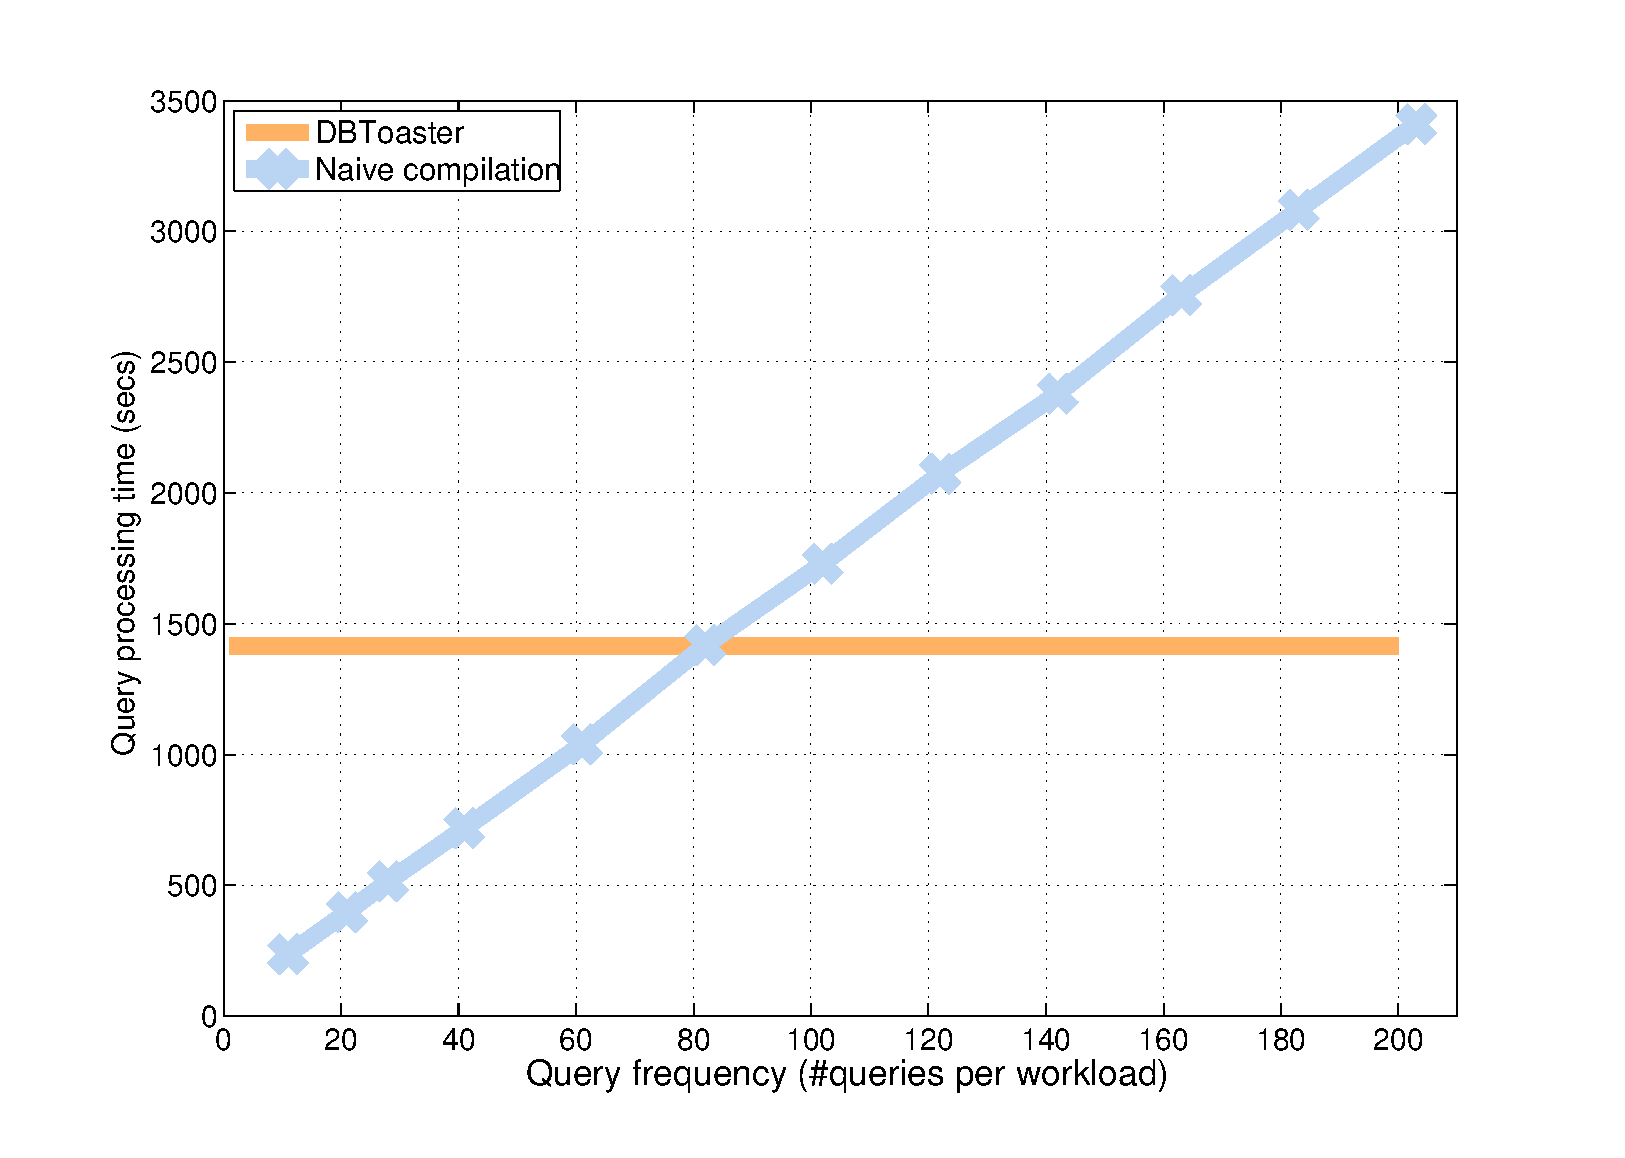
\includegraphics[scale=0.25]{../plots/vwap_query_freq_dn}
\end{center}
\caption{Query frequency limit for VWAP application, indicating the
query execution frequency beyond which DBToaster outperforms the naive query
plan compilation technique.}
\label{fig:vwap_query_freq}
\end{figure}

\begin{figure}
\begin{center}
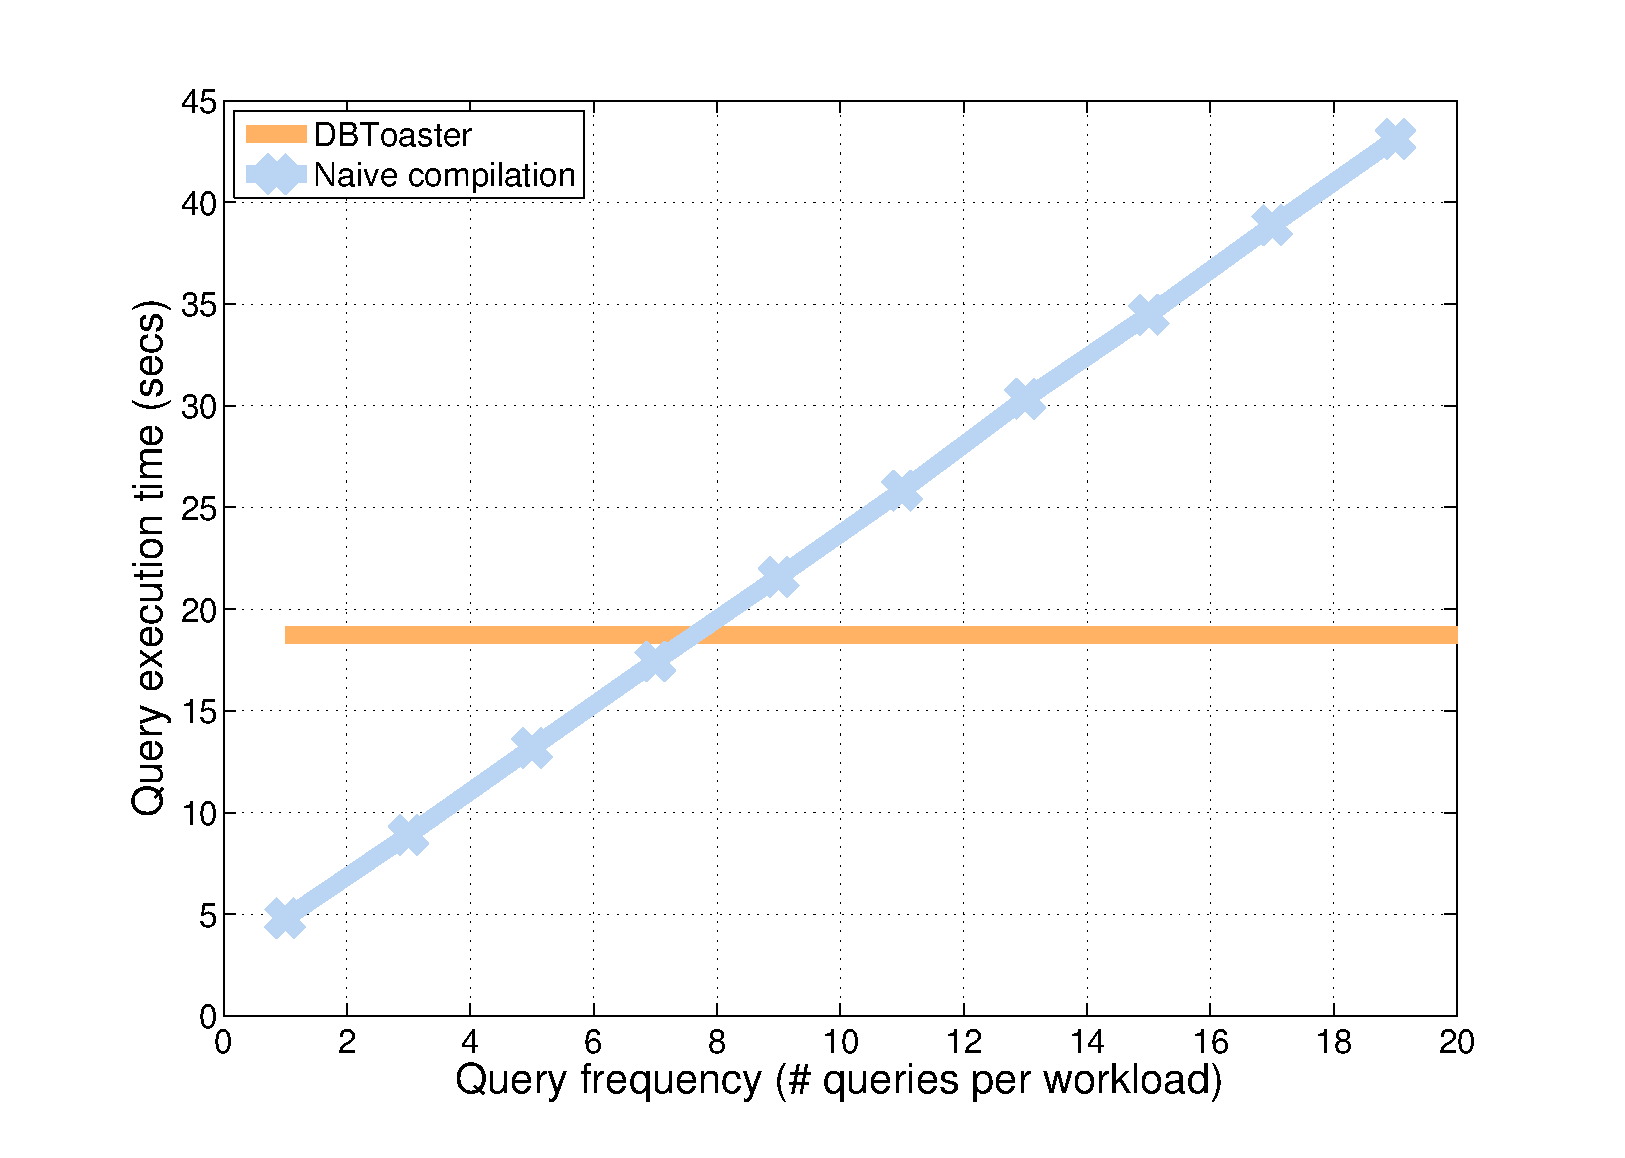
\includegraphics[scale=0.25]{../plots/ssb_query_freq_dn}
\end{center}
\caption{Query frequency limit for warehouse loading application, indicating the
query execution frequency beyond which DBToaster outperforms the naive query
plan compilation technique.}
\label{fig:ssb_query_freq}
\end{figure}

\subsection{Memory Analysis and Batch Execution}


\comment{
Dataset:

\begin{itemize}
  \item TotalView-ITCH dataset: 3 month's worth of MSFT order book messages
  taken from NASDAQ, (~2.2Gb dataset).
  \item Orderbook schema: day, time in us since beginning of day, order id,
  order type, share volume, bid/ask price
\end{itemize}

Queries:

\begin{verbatim}
select * from
  (select ax_bids.mmid, abs(
    sum(ax_bids.volume*
      (act_now.expected_price - ax_bids.price)) -
    sum(ax_asks.volume*
      (ax_asks.price - act_now.expected_price)))
    as ax_bias
  from
    (select mmid, price, volume from bids
       where mmid in axs) as ax_bids,
    (select mmid, price, volume from asks
       where mmid in axs) as ax_asks,
    (select expected_price
        from technical_indicator
        where entrance_condition)
    as act_now
  where ax_bids.mmid = ax_asks.mmid
  group by ax_bids.mmid) as sneaky_ax,
where ax_bias > 10000
\end{verbatim}

Figures:

\begin{enumerate}
  \item Takeaway experiment: end-to-end throughput comparison for a variety of
  insert/update/delete rates. Requires replay speed parameter in data loader.
  Comparison points include Postgres, naive compilation, simple version
  of \compiler, \compiler\ with lazy evaluation, \compiler\ with bulk insert
  mode at 2 or 3 different chunk sizes.

  \item Detail experiment: analyse effect of bulk loading operations compared to
  simple compiler, on a variety of queries, e.g. selectivities and keys.
  Dependent variables for plots: cache hit rates for locality analysis,
  throughput to understand pipelining effects. Is there anything lower lever we
  can do for pipelining?

  \item Detail experiment: selectivity experiment, comparing \compiler\ w/ lazy
  eval, and w/ bulk loading (separately) to next best, for a variety of
  join selectivities and keys.

  \item Detail experiment: space vs recomputation analysis, where we vary the
  maps we keep between extremes of maps from simple decomposition, to full base
  tables.

  \item Quality of compiled code, and compiler effect? e.g. speed provided with
  different -O flags?

\end{enumerate}
}

\section{Conclusion}

\footnotesize{
\bibliographystyle{abbrv}%{plain}
\bibliography{sigmod12-dbtoaster,bibtex}
}

\appendix
\section{Queries}
\label{app:queries}
\vspace{-4mm}
\hspace{-5mm}\vspace{-8mm}
\begin{tabular}{lp{0.95\textwidth}}
\begin{rotate}{90}\hspace{-1cm}\underline{AXF}\end{rotate} &
{\scriptsize
\begin{verbatim}
SELECT   b.broker_id, sum(a.volume + -1 * b.volume)
FROM     bids b, asks a
WHERE    b.broker_id = a.broker_id
  AND    ( (a.price + ((-1) * b.price) > 1000) OR
           (b.price + ((-1) * a.price) > 1000) )
GROUP BY b.broker_id;
\end{verbatim}
}
\end{tabular}

\hspace{-5mm}\vspace{-8mm}
\begin{tabular}{lp{0.95\textwidth}}
\begin{rotate}{90}\hspace{-1cm}\underline{BSP}\end{rotate} &
{\scriptsize
\begin{verbatim}
SELECT x.broker_id, SUM(x.volume * x.price - y.volume * y.price)
FROM   bids x, bids y
WHERE  x.broker_id = y.broker_id AND x.t > y.t GROUP BY x.broker_id;
\end{verbatim}
}
\end{tabular}

\hspace{-5mm}\vspace{-8mm}
\begin{tabular}{lp{0.95\textwidth}}
\begin{rotate}{90}\hspace{-1cm}\underline{BSV}\end{rotate} &
{\scriptsize
\begin{verbatim}
SELECT x.broker_id, SUM(x.volume * x.price * y.volume * y.price * 0.5)
FROM   bids x, bids y
WHERE  x.broker_id = y.broker_id GROUP BY x.broker_id;
\end{verbatim}
}
\end{tabular}

\hspace{-5mm}\vspace{-8mm}
\begin{tabular}{lp{0.95\textwidth}}
\begin{rotate}{90}\hspace{-1cm}\underline{MST}\end{rotate} &
{\scriptsize
\begin{verbatim}
SELECT b.broker_id, sum(a.price*a.volume+-1*b.price*b.volume)
FROM   bids b, asks a
WHERE 0.25*(select sum(a1.volume) from asks a1) >
      (select sum(a2.volume) from asks a2 where a2.price > a.price)
AND   0.25*(select sum(b1.volume) from bids b1) >
      (select sum(b2.volume) from bids b2 where b2.price > b.price)
GROUP BY b.broker_id;
\end{verbatim}
}
\end{tabular}

\hspace{-5mm}\vspace{-8mm}
\begin{tabular}{lp{0.95\textwidth}}
\begin{rotate}{90}\hspace{-0.75cm}\underline{PS}\end{rotate} &
{\scriptsize
\begin{verbatim}
SELECT sum(a.price+-1*b.price) FROM bids b, asks a
WHERE ( b.volume>0.0001*(select sum(b1.volume) from bids b1) )
AND   ( a.volume>0.0001*(select sum(a1.volume) from asks a1) );
\end{verbatim}
}
\end{tabular}

\hspace{-5mm}\vspace{-8mm}
\begin{tabular}{lp{0.95\textwidth}}
\begin{rotate}{90}\hspace{-1.25cm}\underline{VWAP}\end{rotate} &
{\scriptsize
\begin{verbatim}
SELECT sum(b1.price * b1.volume) 
FROM   bids b1
WHERE  0.25 * (select sum(b3.volume) from bids b3) >
       (select sum(b2.volume) from bids b2 where b2.price > b1.price);
\end{verbatim}
}
\end{tabular}

\hspace{-5mm}\vspace{-8mm}
\begin{tabular}{lp{0.95\textwidth}}
\begin{rotate}{90}\hspace{-0.75cm}\underline{Q3}\end{rotate} &
{\scriptsize
\begin{verbatim}
SELECT ORDERS.orderkey, ORDERS.orderdate, ORDERS.shippriority,
       SUM(extendedprice * (1 - discount))
FROM   CUSTOMER, ORDERS, LINEITEM
WHERE  CUSTOMER.mktsegment = 'BUILDING'
  AND  ORDERS.custkey = CUSTOMER.custkey
  AND  LINEITEM.orderkey = ORDERS.orderkey
  AND  ORDERS.orderdate < DATE('1995-03-15')
  AND  LINEITEM.SHIPDATE > DATE('1995-03-15')
GROUP BY ORDERS.orderkey, ORDERS.orderdate, ORDERS.shippriority;
\end{verbatim}}
\end{tabular}

\hspace{-5mm}\vspace{-8mm}
\begin{tabular}{lp{0.95\textwidth}}
\begin{rotate}{90}\hspace{-0.9cm}\underline{Q11}\end{rotate} &
{\scriptsize
\begin{verbatim}
SELECT ps.partkey, sum(ps.supplycost * ps.availqty)
FROM   partsupp ps, supplier s
WHERE  ps.suppkey = s.suppkey GROUP BY ps.partkey;
\end{verbatim}}
\end{tabular}

\hspace{-5mm}\vspace{-8mm}
\begin{tabular}{lp{0.95\textwidth}}
\begin{rotate}{90}\hspace{-0.9cm}\underline{Q17}\end{rotate} &
{\scriptsize
\begin{verbatim}
SELECT sum(l.extendedprice) FROM lineitem l, part p
WHERE  p.partkey = l.partkey
AND    l.quantity < 0.005*
       (SELECT sum(l2.quantity)
        FROM lineitem l2 WHERE l2.partkey = p.partkey);
\end{verbatim}}
\end{tabular}

\hspace{-5mm}\vspace{-8mm}
\begin{tabular}{lp{0.95\textwidth}}
\begin{rotate}{90}\hspace{-0.9cm}\underline{Q18}\end{rotate} &
{\scriptsize
\begin{verbatim}
SELECT c.custkey, sum(l1.quantity)
FROM customer c, orders o, lineitem l1
WHERE 1 <= (SELECT sum(1) FROM lineitem l2
            WHERE l1.orderkey = l2.orderkey
            AND 100 < (SELECT sum(l3.quantity) FROM lineitem l3
                       WHERE l2.orderkey = l3.orderkey))
AND c.custkey = o.custkey AND o.orderkey = l1.orderkey
GROUP BY c.custkey;
\end{verbatim}}
\end{tabular}

\hspace{-5mm}\vspace{-8mm}
\begin{tabular}{lp{0.95\textwidth}}
\begin{rotate}{90}\hspace{-0.9cm}\underline{Q22}\end{rotate} &
{\scriptsize
\begin{verbatim}
SELECT c1.nationkey, sum(c1.acctbal) FROM customer c1
WHERE c1.acctbal <
    (SELECT sum(c2.acctbal) FROM customer c2 WHERE c2.acctbal > 0)
AND 0 = (SELECT sum(1) FROM orders o WHERE o.custkey = c1.custkey)
GROUP BY c1.nationkey
\end{verbatim}}
\end{tabular}

\comment{
\hspace{-5mm}\vspace{-8mm}
\begin{tabular}{lp{0.95\textwidth}}
\begin{rotate}{90}\hspace{-0.9cm}\underline{SVL}\end{rotate} &
{\scriptsize
\begin{verbatim}
SELECT s1.rackid, SUM(1) FROM Server s1
WHERE (SELECT SUM(s2.load) FROM Server s2) * 1.5
      < (SELECT SUM(1) FROM Server s3) * s1.load
GROUP BY s1.rackid;
\end{verbatim}}
\end{tabular}
}

\hspace{-5mm}\vspace{-8mm}
\begin{tabular}{lp{0.95\textwidth}}
\begin{rotate}{90}\hspace{-1.1cm}\underline{SSB4}\end{rotate} &
{\scriptsize
\begin{verbatim}
SELECT sn.regionkey, cn.regionkey, PART.type, SUM(LINEITEM.quantity)
FROM   CUSTOMER, ORDERS, LINEITEM, PART, SUPPLIER, NATION cn, NATION sn
WHERE  CUSTOMER.custkey = ORDERS.custkey
  AND  ORDERS.orderkey = LINEITEM.orderkey
  AND  PART.partkey = LINEITEM.partkey
  AND  SUPPLIER.suppkey = LINEITEM.suppkey
  AND  ORDERS.orderdate >= DATE('1997-01-01')
  AND  ORDERS.orderdate <  DATE('1998-01-01')
  AND  cn.nationkey = CUSTOMER.nationkey
  AND  sn.nationkey = SUPPLIER.nationkey
GROUP BY sn.regionkey, cn.regionkey, PART.type
\end{verbatim}}
\end{tabular}


\end{document}

